\chapter{User Study}

We conducted a user study in order to do the following: (1) test the usability of firefly, and (2) discover the human factors that children exhibit when using a sandbox mobile musical tool. The user study involved several phases namely (1) Participant Recruitment, (2) usability tests, (3) post testing, (4) expert evaluation and (5) analysis of data. Each phase is described in the succeeding sections. 

% \section{Music Tasks}
%\section{FireflyX Testing}
\section{Participants}
Children between the age of five to eight years old were recruited. These participants were recruited using  convenience sampling. We collected specific information from the participants such as gender, age, prior training in music and handedness. These details could be seen in Table \ref{tab:ParticipantDemographic}. Prior knowledge in music was categorized between none to familiar. None being no prior knowledge in music at all. Minimal. being the child has seen music notes but could not recognize them individually. Slightly Familiar, being the child can recognize rhythm and pitches present in FireflyX but have not memorized it. Familiar, being the child has memorized the notes, rhythm, and pitches present in FireflyX. Due to the covid-19 pandemic, participant recruitment and testing has to be done online and remotely. As such, locations of participants did not matter as long as timezones allowed them to participate. 

We were able to initially recruit 14 participants through our sampling method. Only 8 out of the original 14 attended the orientation after they were contacted.  Only 6 were able to successfully install the mobile app remotely. The other 2 encountered hardware problems that made them unable to participate any further. Five (5) participants were able to successfully finish the test protocol while the sixth participant decided to withdraw from the study. 

%It is also notable that the first participant lived outside of SEA region which is not covered by the database service we used, this meant that we had to observe him using the application and listen to his outputs closely to be able to replicate it.

%In order to conduct the testing, we recruited four participants through convenience sampling, while ten participants signed up by using a google form. Only eight out of the fourteen total participants agreed to have the orientation. Out of the eight that attended the orientation only 6 were able to install FireflyX, while the other two participants could not install FireflyX due to hardware problems. Five participants were able to finish the tasks, and the sixth participant backed out from participating.

\begin{table}[]
\begin{tabular}{|l|r|l|l|l|}
\hline
Participant Number & \multicolumn{1}{l|}{Age} & Sex    & Dominant Hand & Prior Knowledge in Music \\ \hline
P1      & 7                        & Male   & Right Hand    & None                     \\ \hline
P2      & 8                        & Male   & Left Hand     & Minimal                  \\ \hline
P3      & 6                        & Female & Right Hand    & Minimal                  \\ \hline
P4      & 6                        & Male   & Right Hand     & None                     \\ \hline
P5      & 8                        & Male   & Right Hand    & Slightly Familiar        \\ \hline
\end{tabular}
\caption{Participant Demographic}
\label{tab:ParticipantDemographic}
\end{table}

\section{Testing Protocol}
Due to the complications brought by the covid-19 pandemic, the testing protocol from the first and second iteration were not operationally-feasible. This meant that we had to rely on testing the application remotely. This was done by deploying the latest version of FireflyX via TestFlight. Participants are scheduled into several sessions such as orientation session, task sessions and post testing sessions. Participants will be given instructions and preparations during the orientation session. The app will be installed and downloaded to the devices of the participants remotely. In task sessions, the participants will undergo usability testing while performing the pre-designed tasks in the next sections. There will be five (5) tasks that are progressing in terms of difficulty. These tasks were designed with the help of our music experts and early childhood music teachers. In the post-testing session, the participants will be interviewed and asked to evaluate FireflyX using AttrakDiff. 

The orientation given to the participants and their guardians mainly focused on discussing their rights as a participant, the motivation of our research, the objective of our research, and the tasks that will be given to the child. Profiling of the child is also done at this part. After these, if time is still sufficient, we ask the child to do the first task which is to explore and play with the application. During this, we guided the child on how to compose the alphabet song while teaching them the different functions of the app. The music sheet for the alphabet song can be seen in Figure \ref{fig:AlphabetMusicSheet}
\begin{figure}[H]
    \centering
    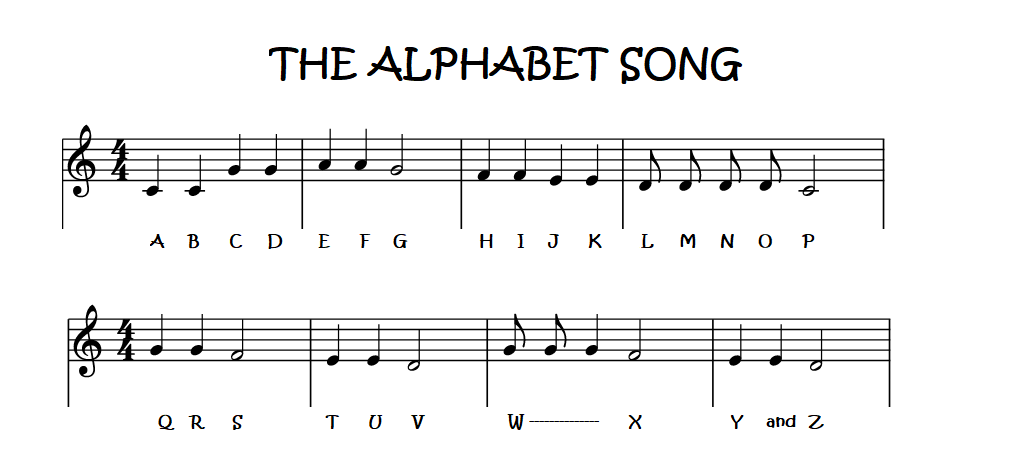
\includegraphics[width=12cm]{figures/NewFigures/alphabetsongmusicsheet.png}
    \caption{The Alphabet Song Music Sheet}
    \label{fig:AlphabetMusicSheet}
\end{figure}
The second task given to the child aims to familiarize them with the different rhythm and patterns present in music. The child is asked to compose the basic rhythm sheet which can be seen in Figure \ref{fig:BasicRhythmMusicSheet}. The child is also given an audio file which they can listen to, in addition to the different visual tips which can be seen in Figure \ref{fig:BasicRhythmTip1} to Figure \ref{fig:BasicRhythmTip5}. The child is expected to finish the task with minimal guidance given to them by their guardians. No other forms of intervention that help the children will be given other than referring them to the tips and guides provided. 

\begin{figure}[H]
    \centering
    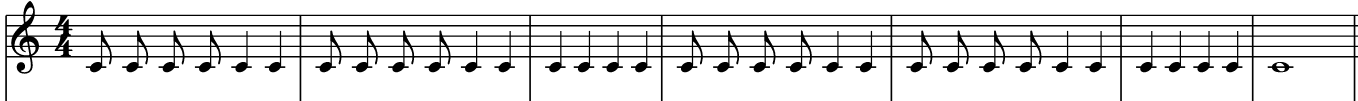
\includegraphics[width=16cm]{figures/NewFigures/BasicRhythmMusicSheet.png}
    \caption{Basic Rhythm Music Sheet}
    \label{fig:BasicRhythmMusicSheet}
\end{figure}

\begin{figure}[H]
    \centering
    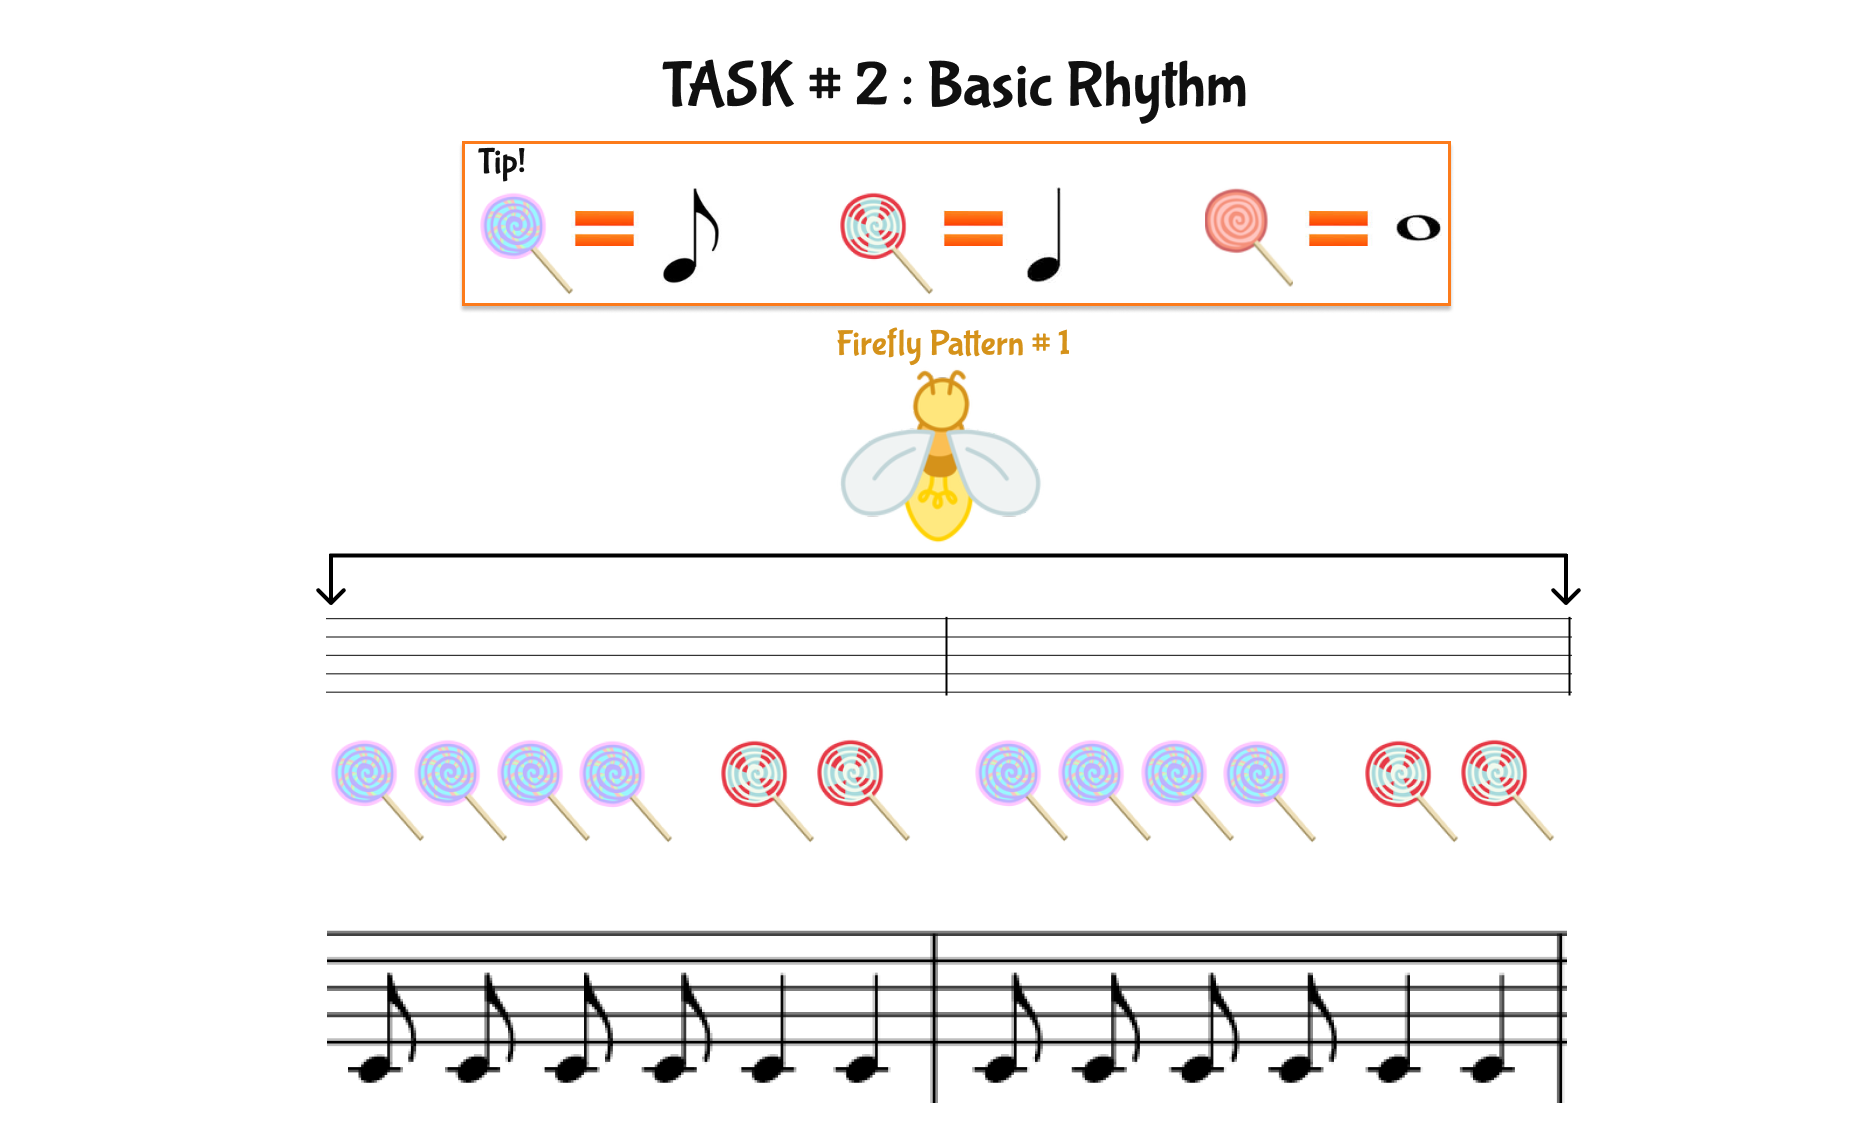
\includegraphics[width=12cm]{figures/NewFigures/BasicRhythmTip1.png}
    \caption{Basic Rhythm Tip 1}
    \label{fig:BasicRhythmTip1}
\end{figure}

\begin{figure}[H]
    \centering
    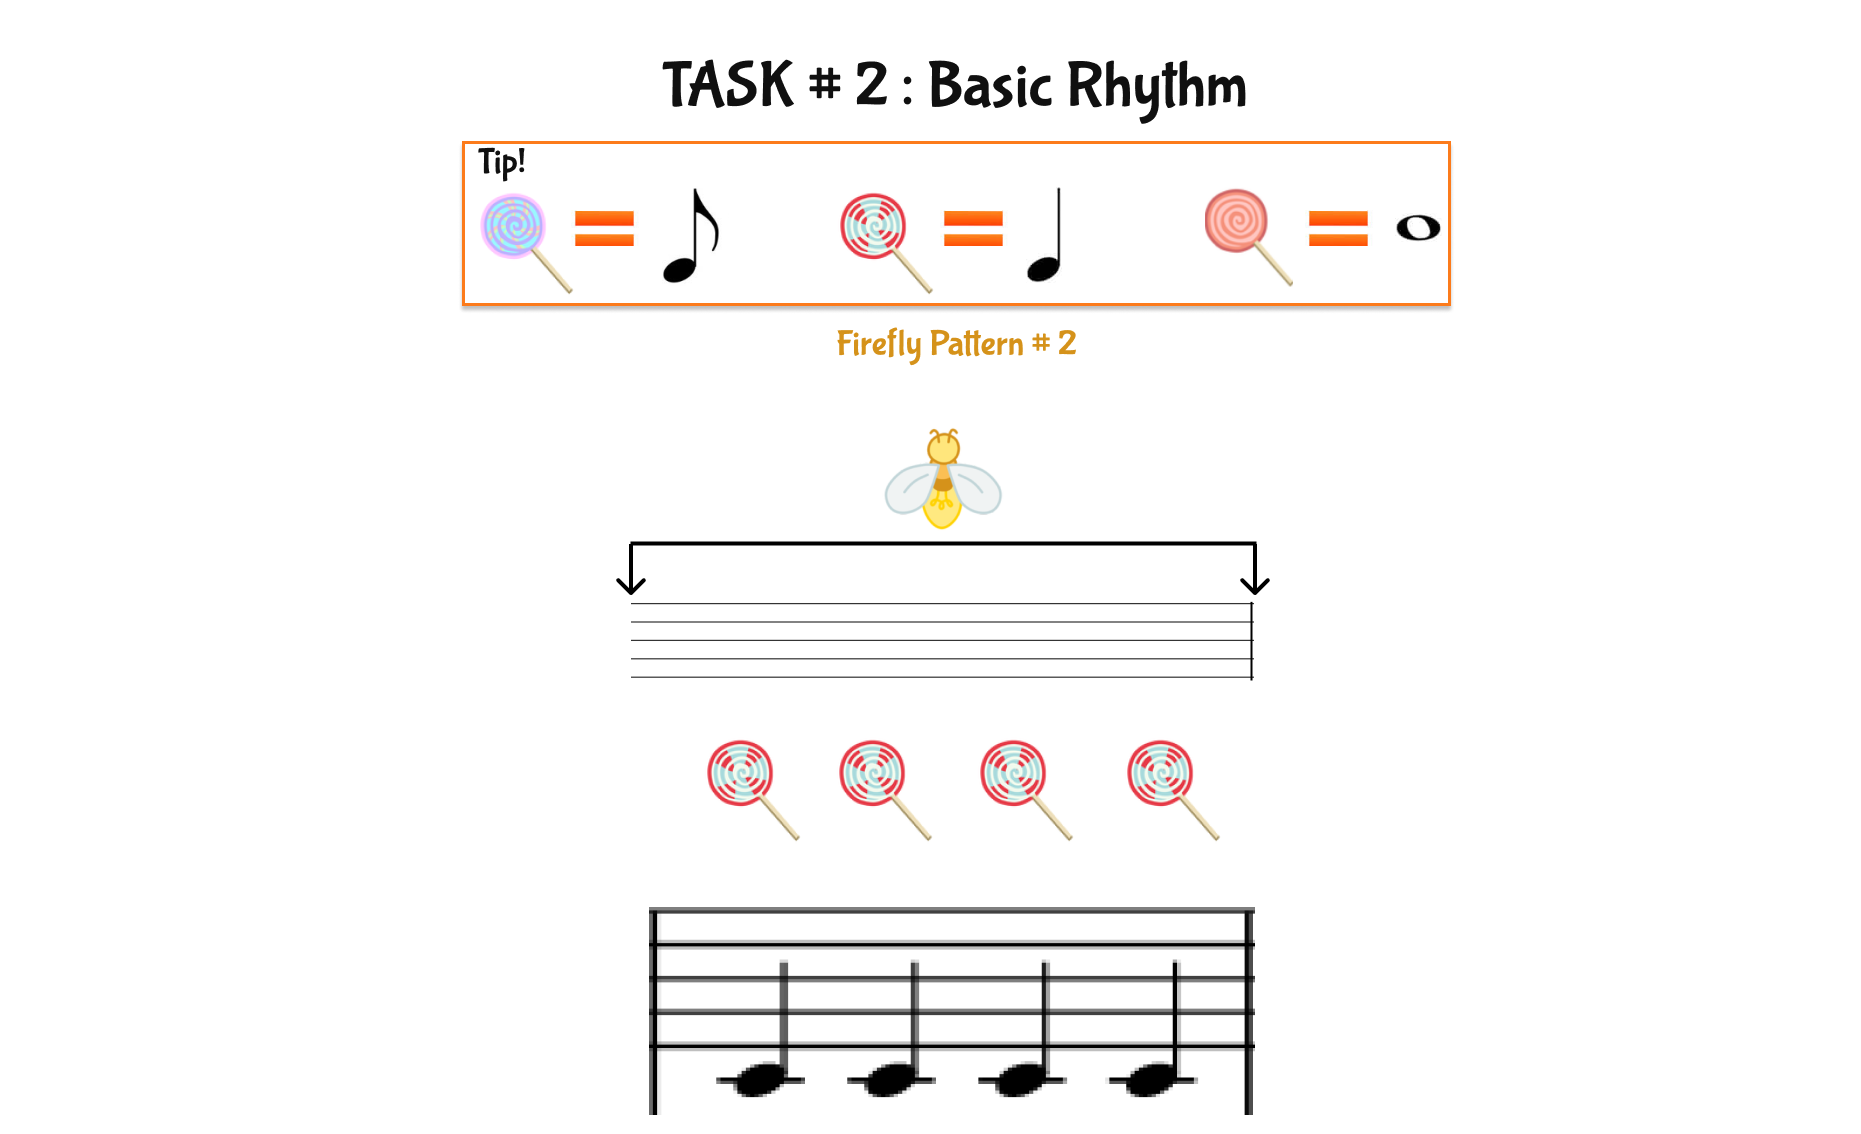
\includegraphics[width=15cm]{figures/NewFigures/BasicRhythmTip2.png}
    \caption{Basic Rhythm Tip 2}
    \label{fig:BasicRhythmTip2}
\end{figure}

\begin{figure}[H]
    \centering
    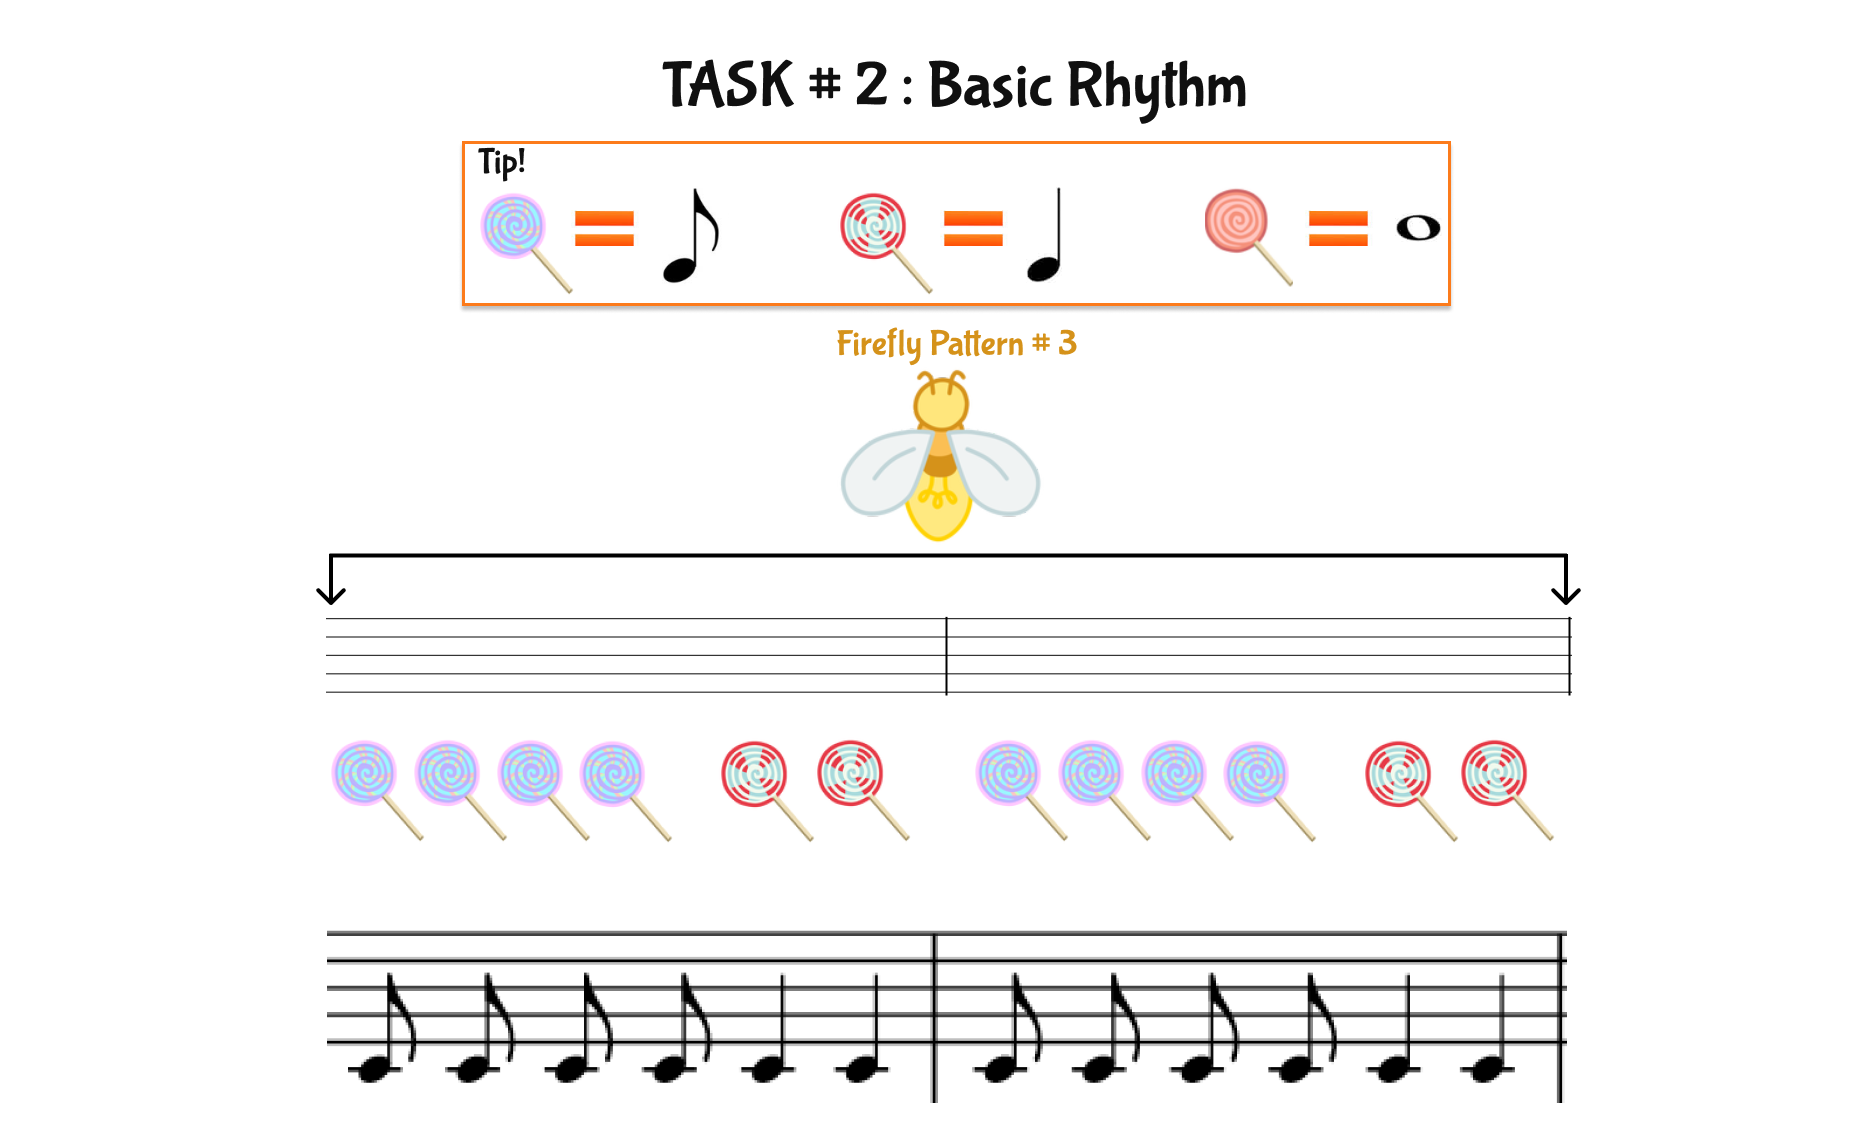
\includegraphics[width=15cm]{figures/NewFigures/BasicRhythmTip3.png}
    \caption{Basic Rhythm Tip 3}
    \label{fig:BasicRhythmTip3}
\end{figure}

\begin{figure}[H]
    \centering
    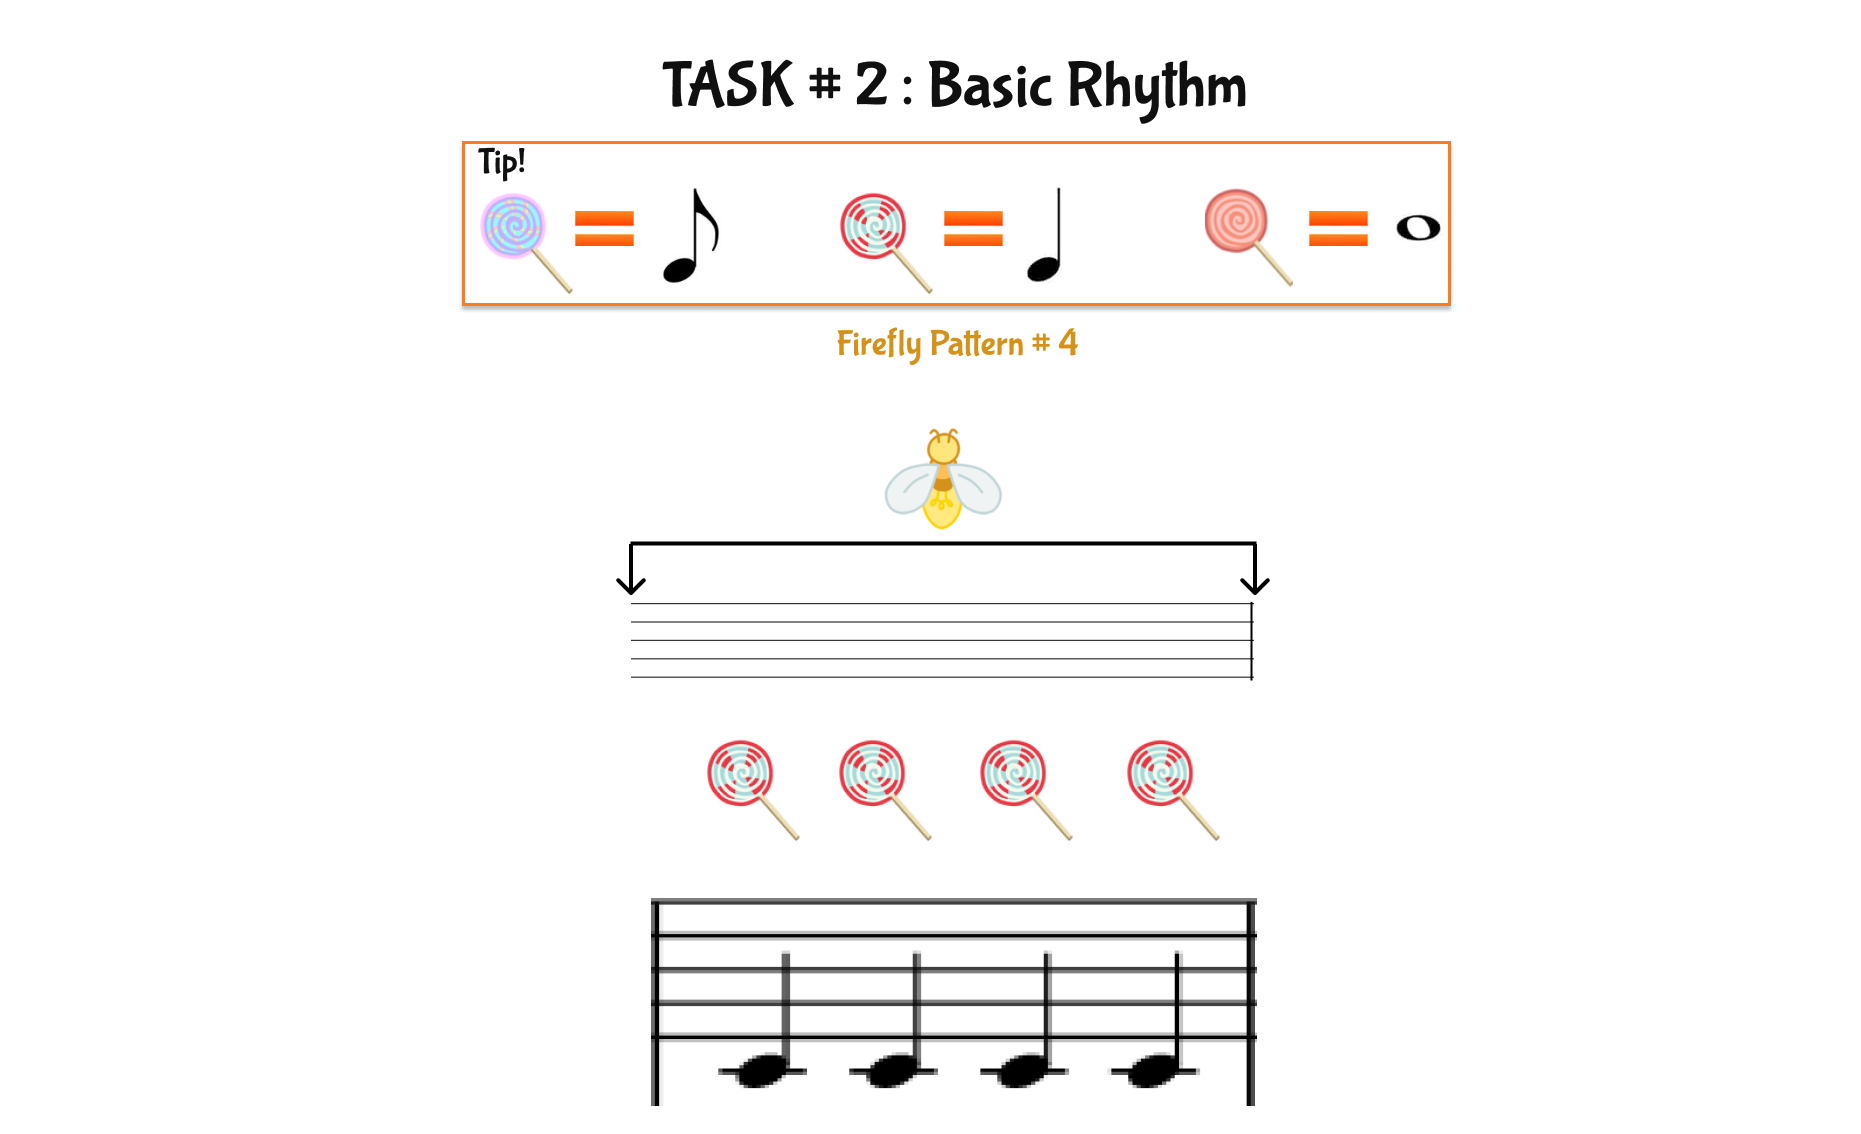
\includegraphics[width=15cm]{figures/NewFigures/BasicRhythmTip4.png}
    \caption{Basic Rhythm Tip 4}
    \label{fig:BasicRhythmTip4}
\end{figure}

\begin{figure}[H]
    \centering
    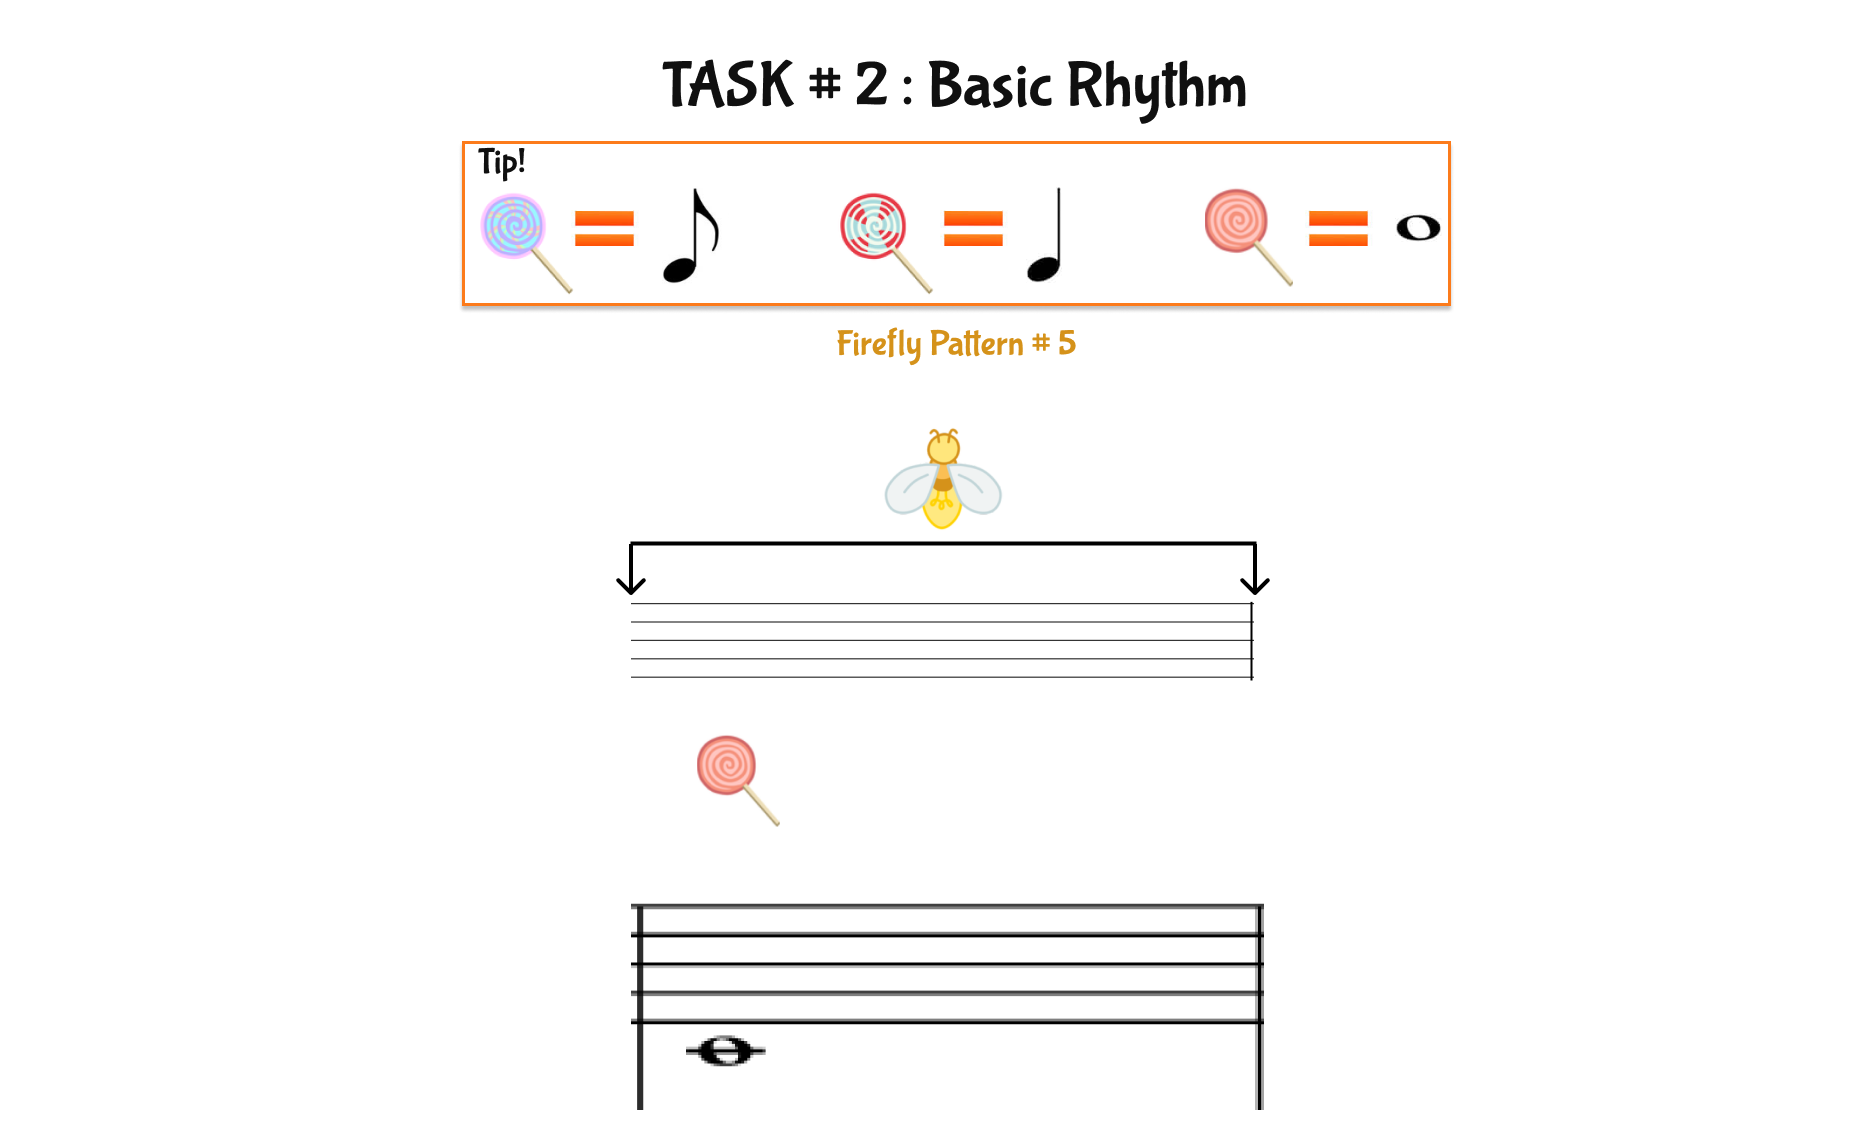
\includegraphics[width=15cm]{figures/NewFigures/BasicRhythmTip5.png}
    \caption{Basic Rhythm Tip 5}
    \label{fig:BasicRhythmTip5}
\end{figure}

The third task given to the child aims to familiarize the them with the usable pitch in the application. Similar with task 2, the child is asked to compose the basic pitch sheet which can be seen in Figure \ref{fig:BasicPitchMusicSheet}. The child is given an audio file which they can listen to, in addition to the visual tips which can be seen in Figure \ref{fig:BasicPitchTip1} to Figure \ref{fig:BasicPitchTip10}. Like in task 2, the child should be able to finish the task with minimal guidance from their guardians. We are also expected to not give any advice or help aside from referring them to the tips given to them.

\begin{figure}[H]
    \centering
    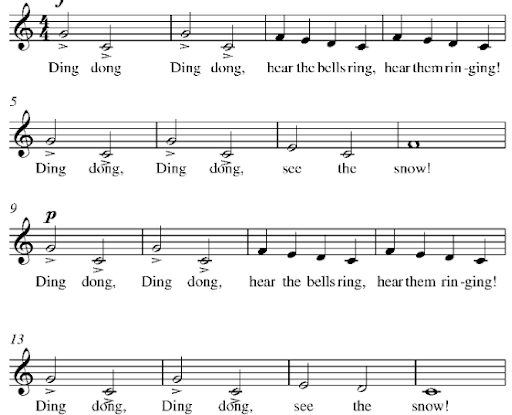
\includegraphics[width=12cm]{figures/NewFigures/BasicPitchMusicSheet.png}
    \caption{Basic Pitch Music Sheet}
    \label{fig:BasicPitchMusicSheet}
\end{figure}

\begin{figure}[H]
    \centering
    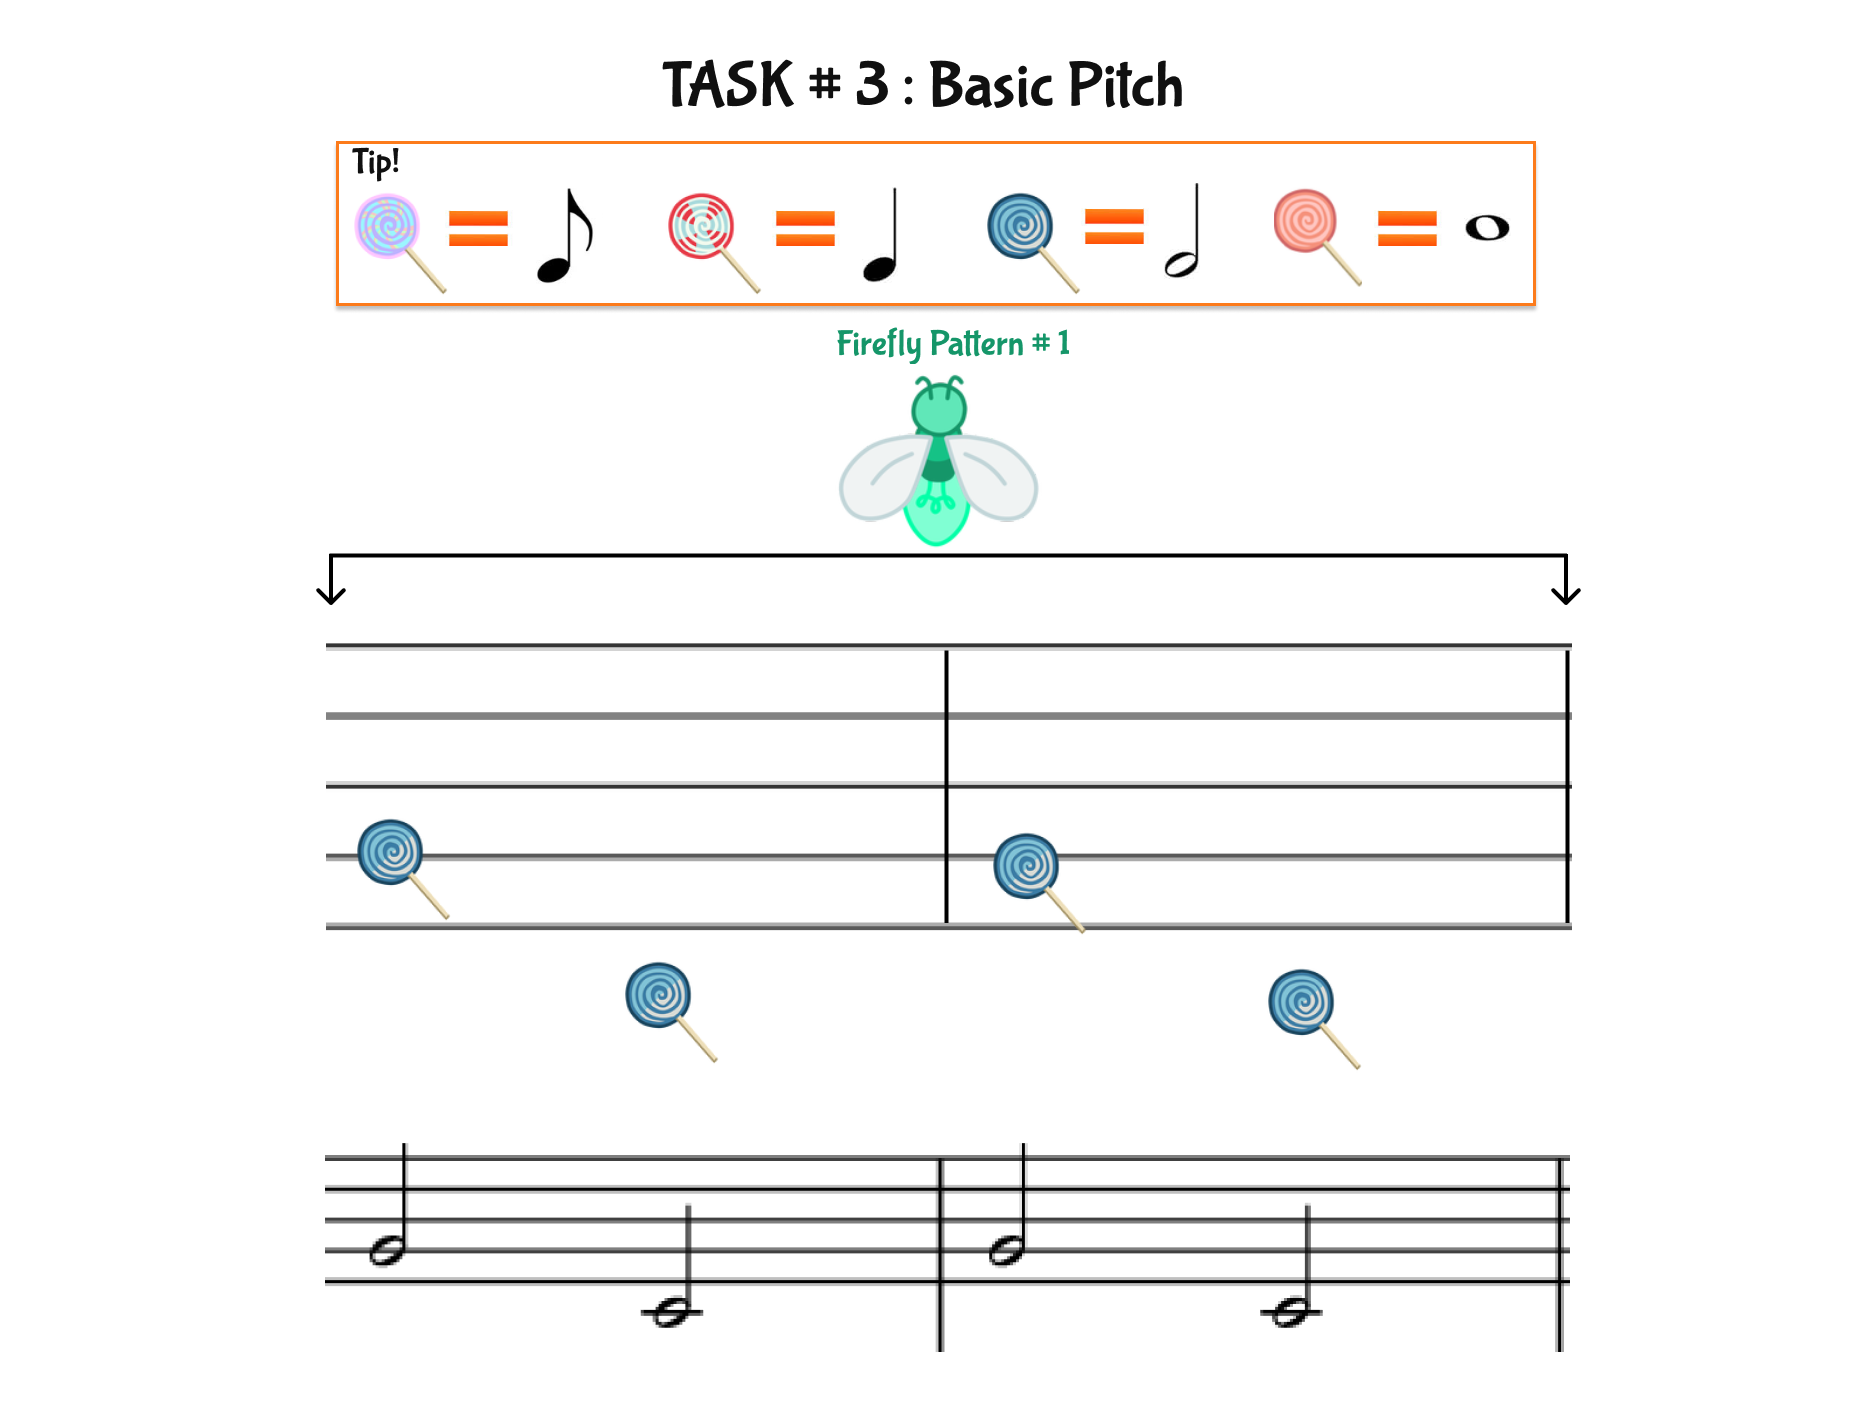
\includegraphics[width=12cm]{figures/NewFigures/BasicPitchTip1.png}
    \caption{Basic Pitch Tip 1}
    \label{fig:BasicPitchTip1}
\end{figure}

\begin{figure}[H]
    \centering
    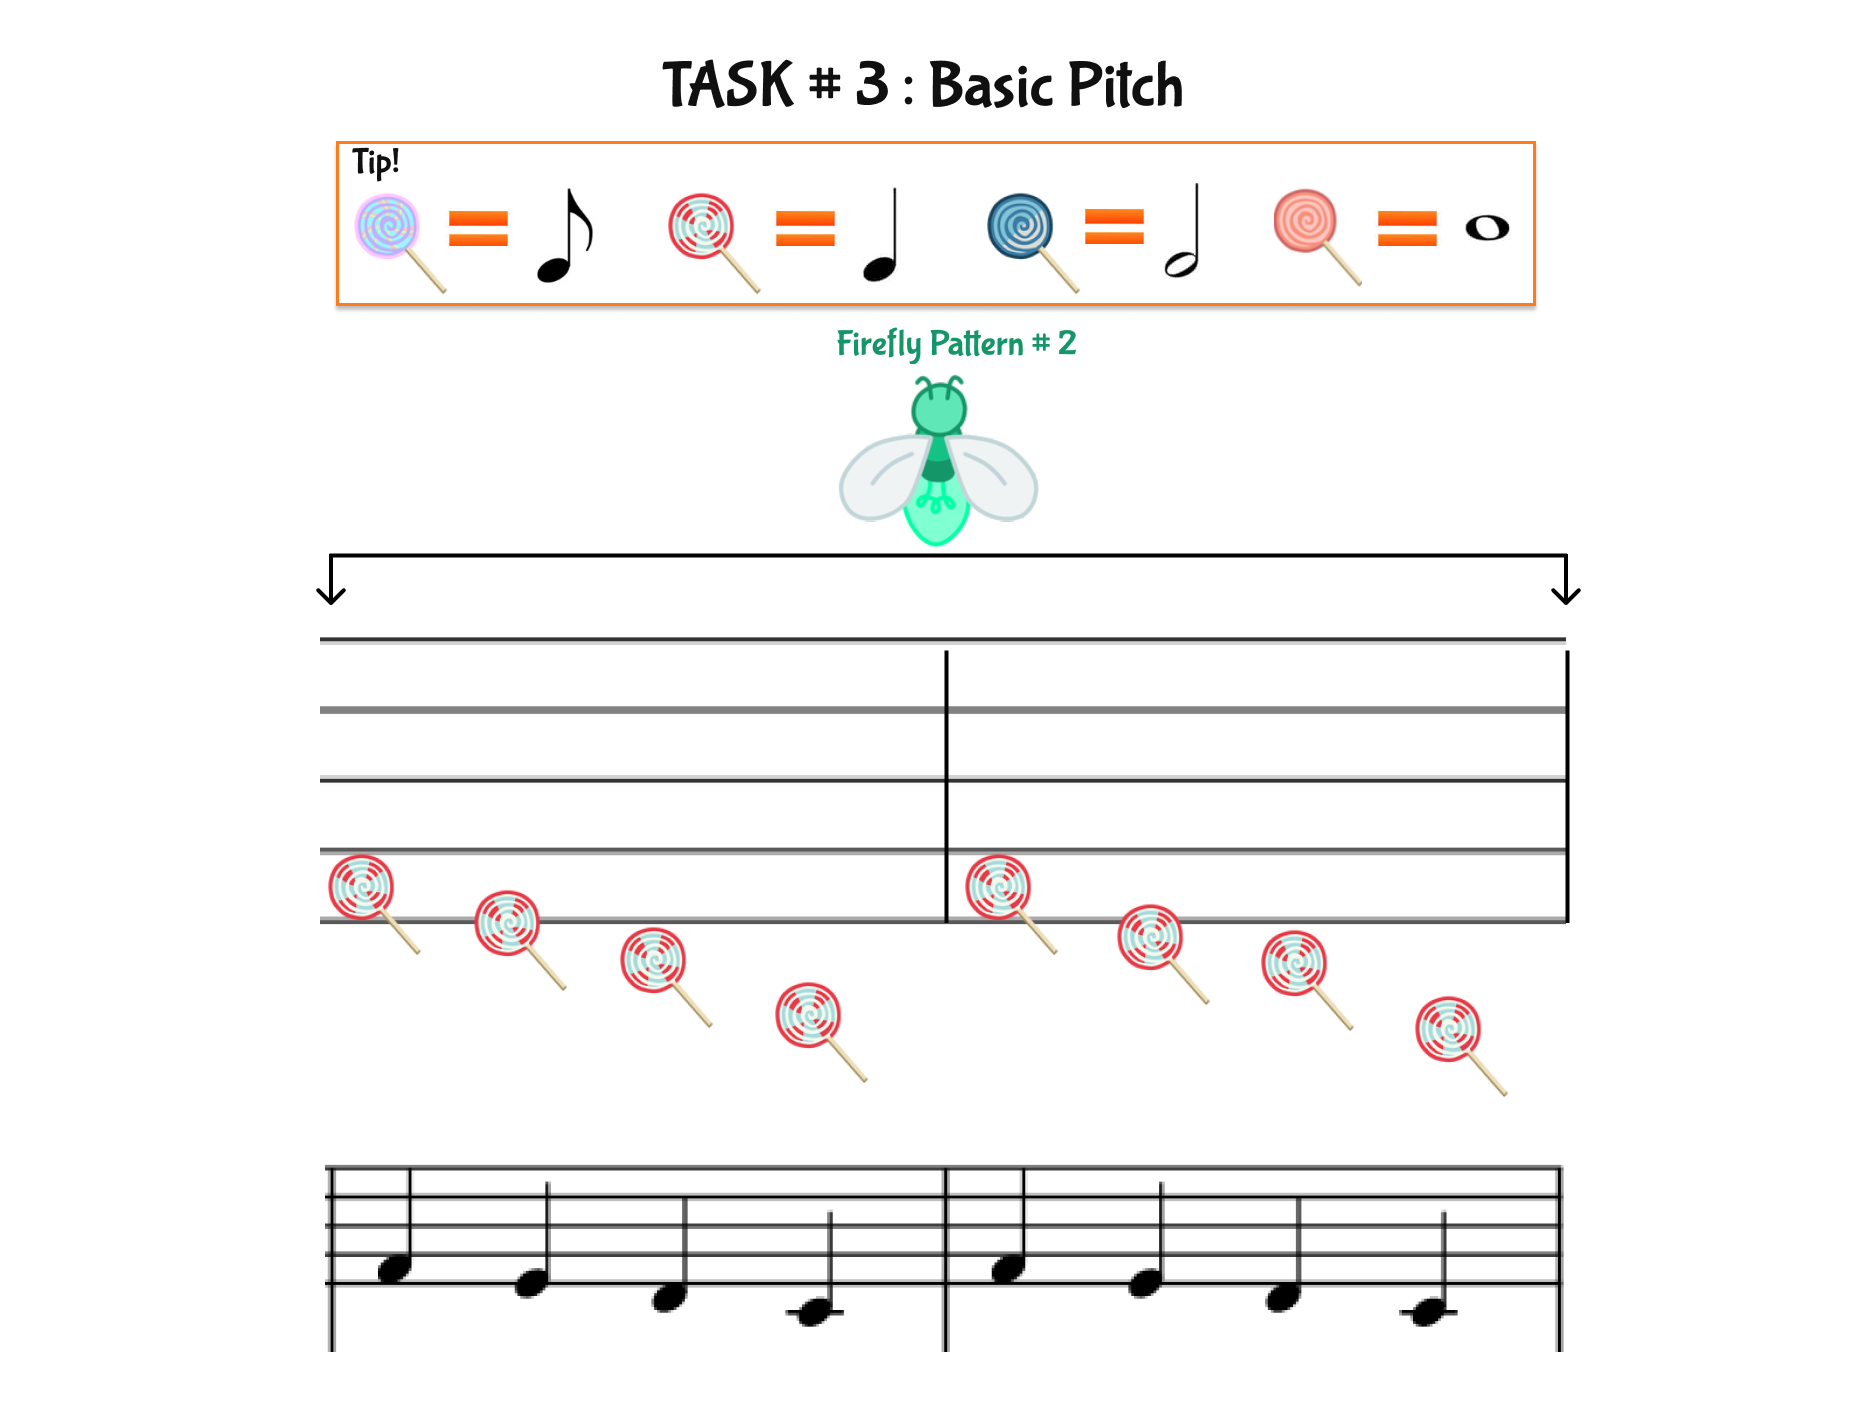
\includegraphics[width=12cm]{figures/NewFigures/BasicPitchTip2.png}
    \caption{Basic Pitch Tip 2}
    \label{fig:BasicPitchTip2}
\end{figure}

\begin{figure}[H]
    \centering
    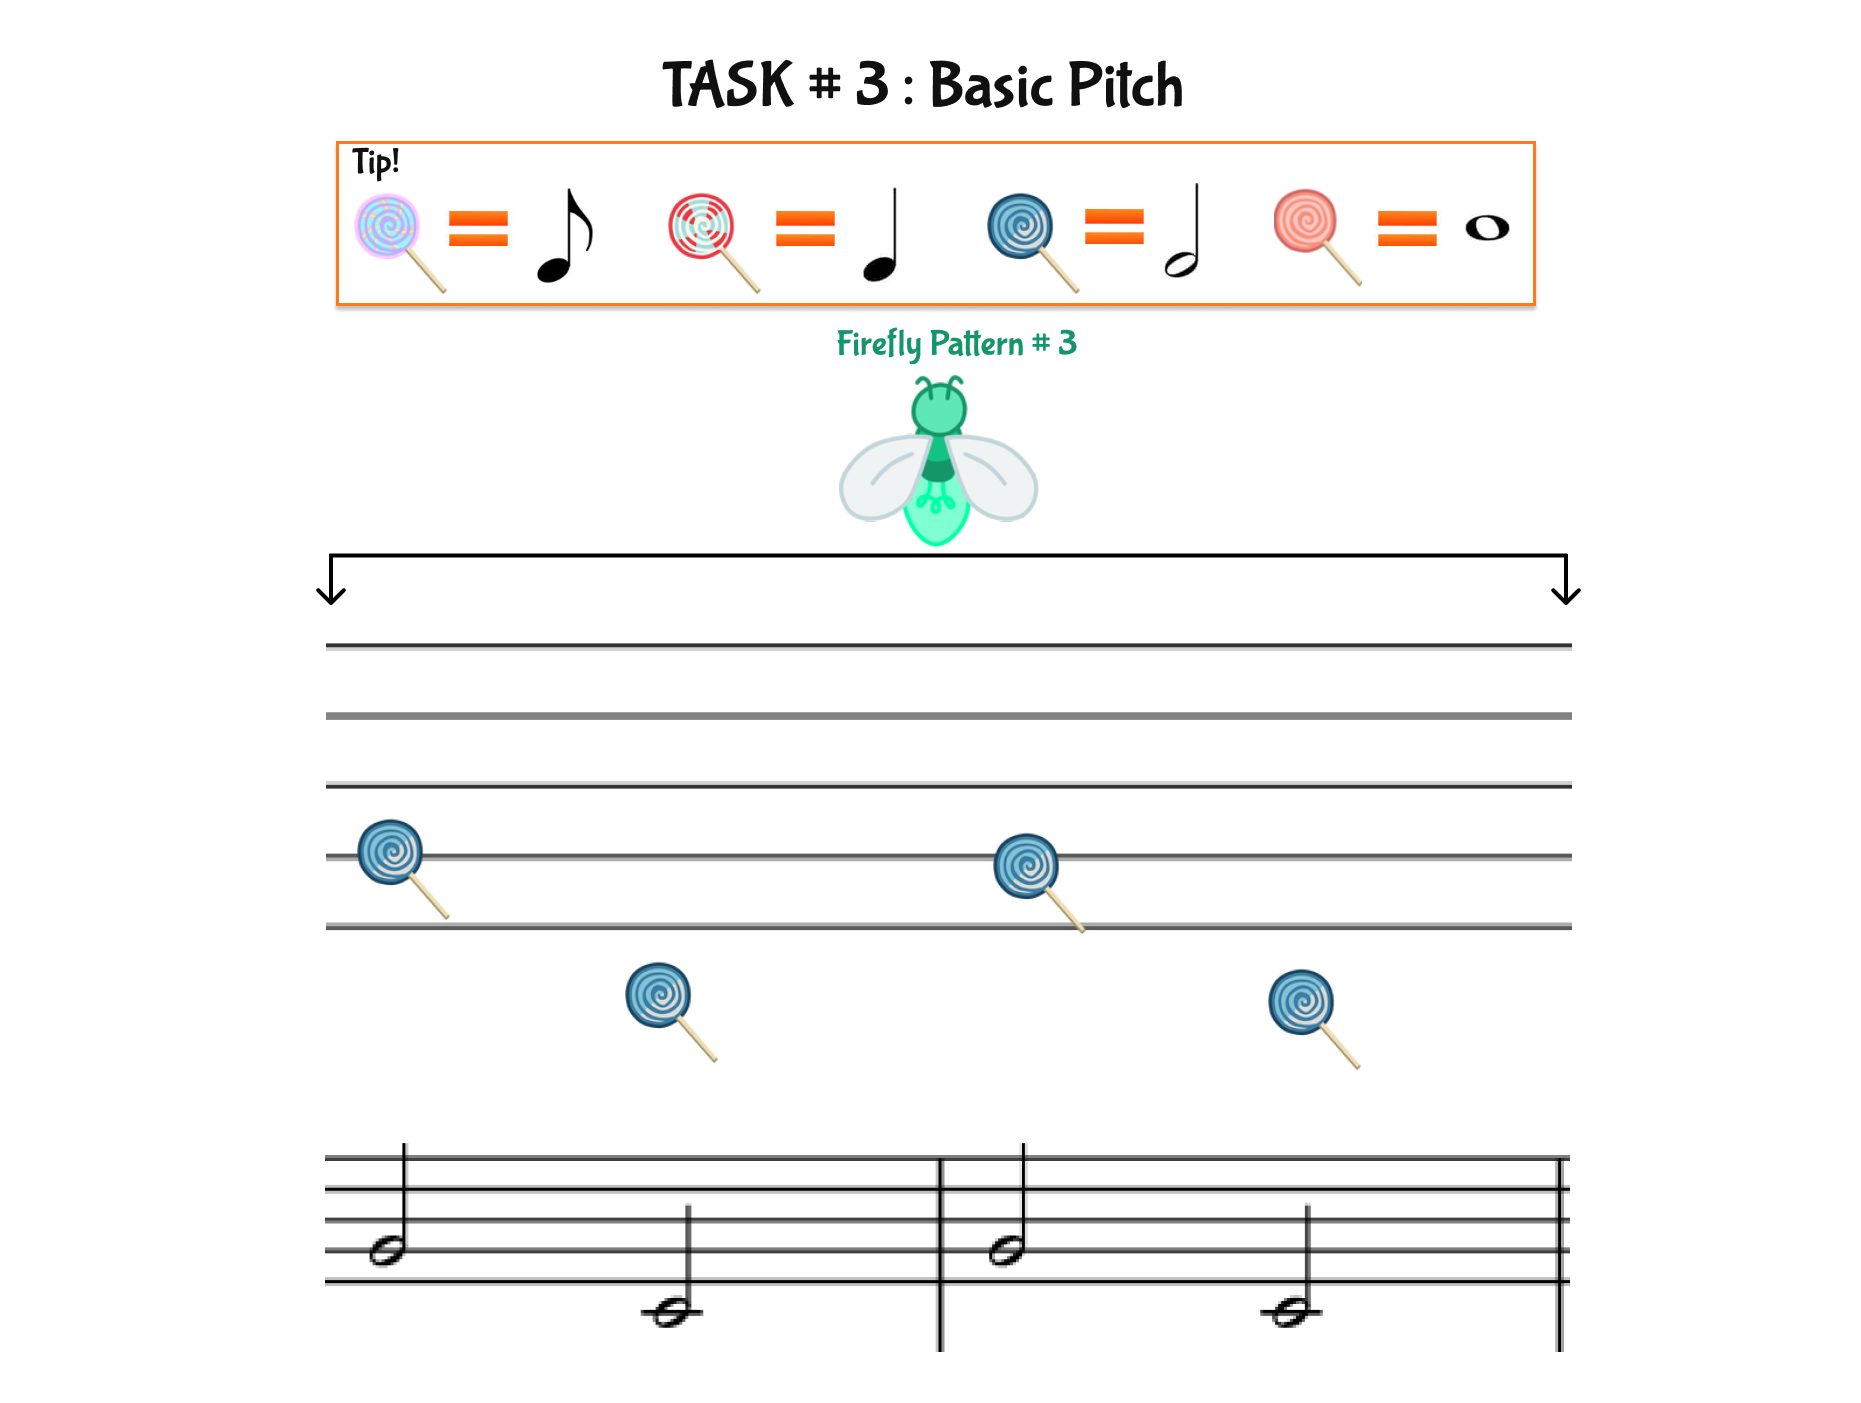
\includegraphics[width=12cm]{figures/NewFigures/BasicPitchTip3.png}
    \caption{Basic Pitch Tip 3}
    \label{fig:BasicPitchTip3}
\end{figure}

\begin{figure}[H]
    \centering
    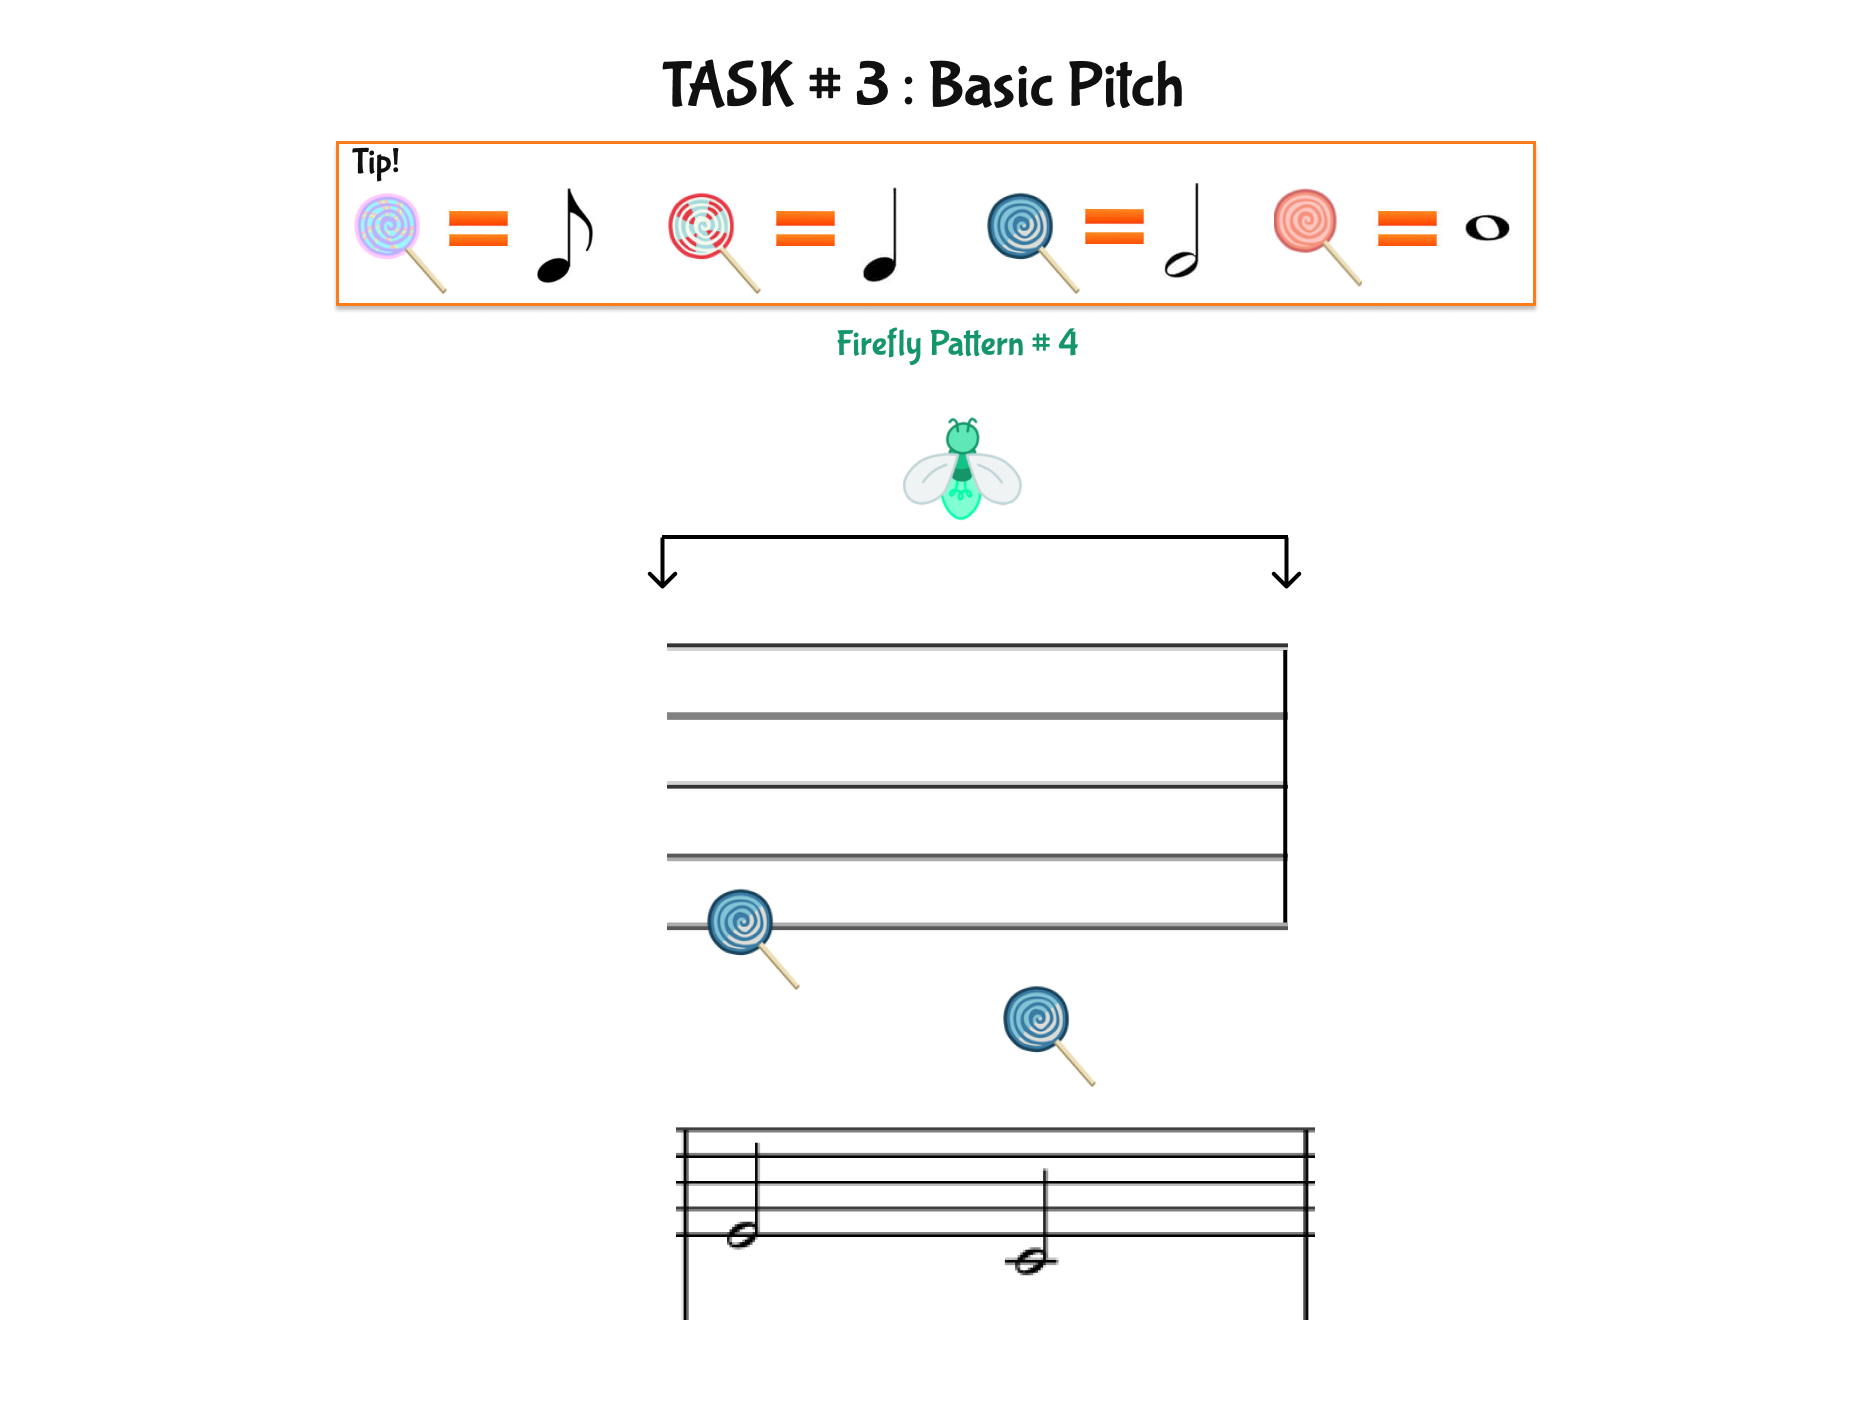
\includegraphics[width=12cm]{figures/NewFigures/BasicPitchTip4.png}
    \caption{Basic Pitch Tip 4}
    \label{fig:BasicPitchTip4}
\end{figure}

\begin{figure}[H]
    \centering
    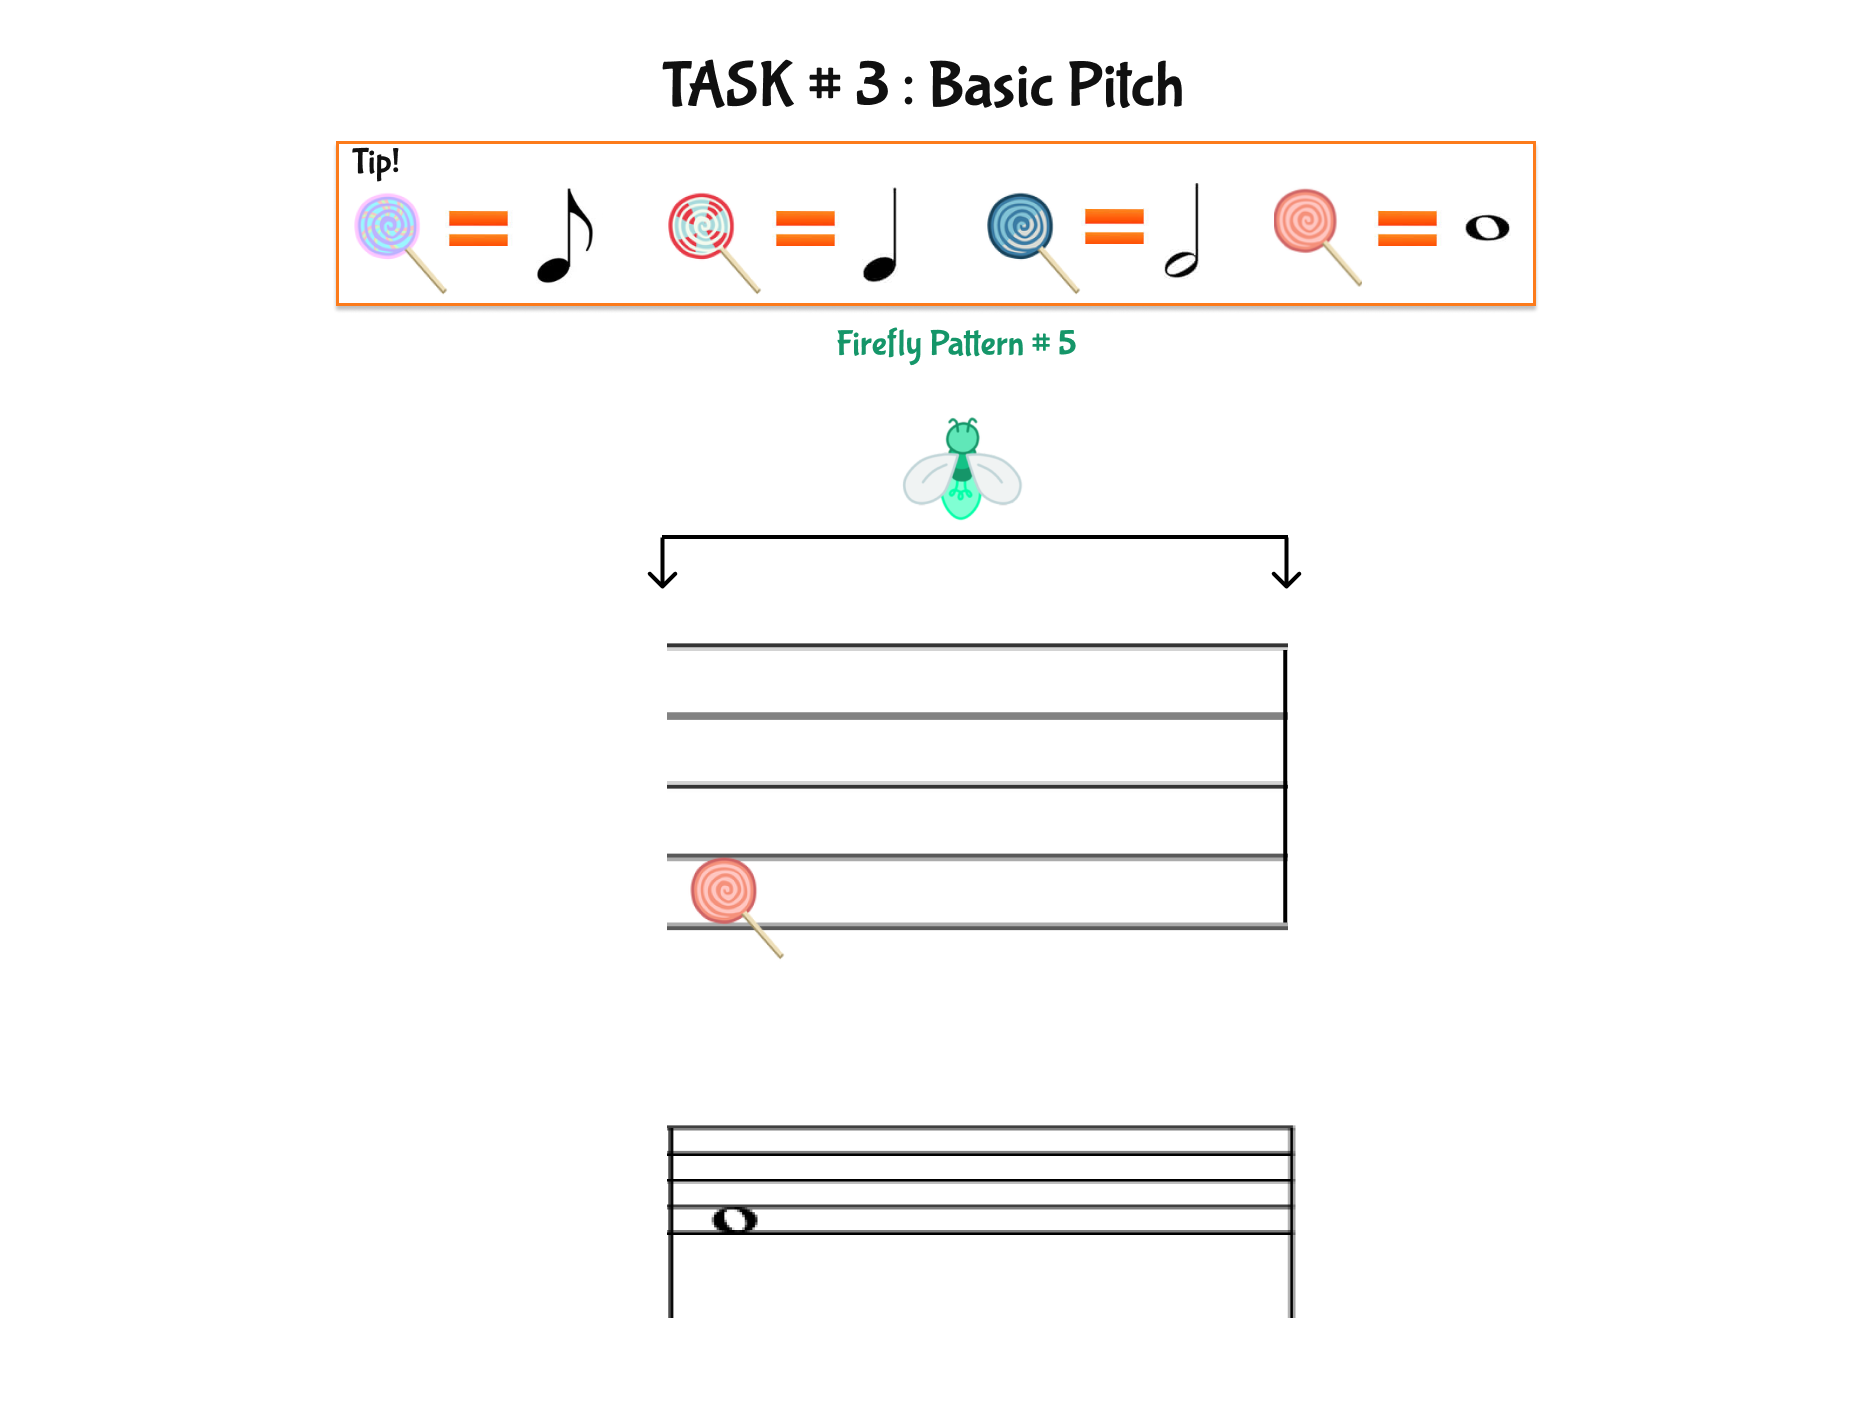
\includegraphics[width=12cm]{figures/NewFigures/BasicPitchTip5.png}
    \caption{Basic Pitch Tip 5}
    \label{fig:BasicPitchTip5}
\end{figure}

\begin{figure}[H]
    \centering
    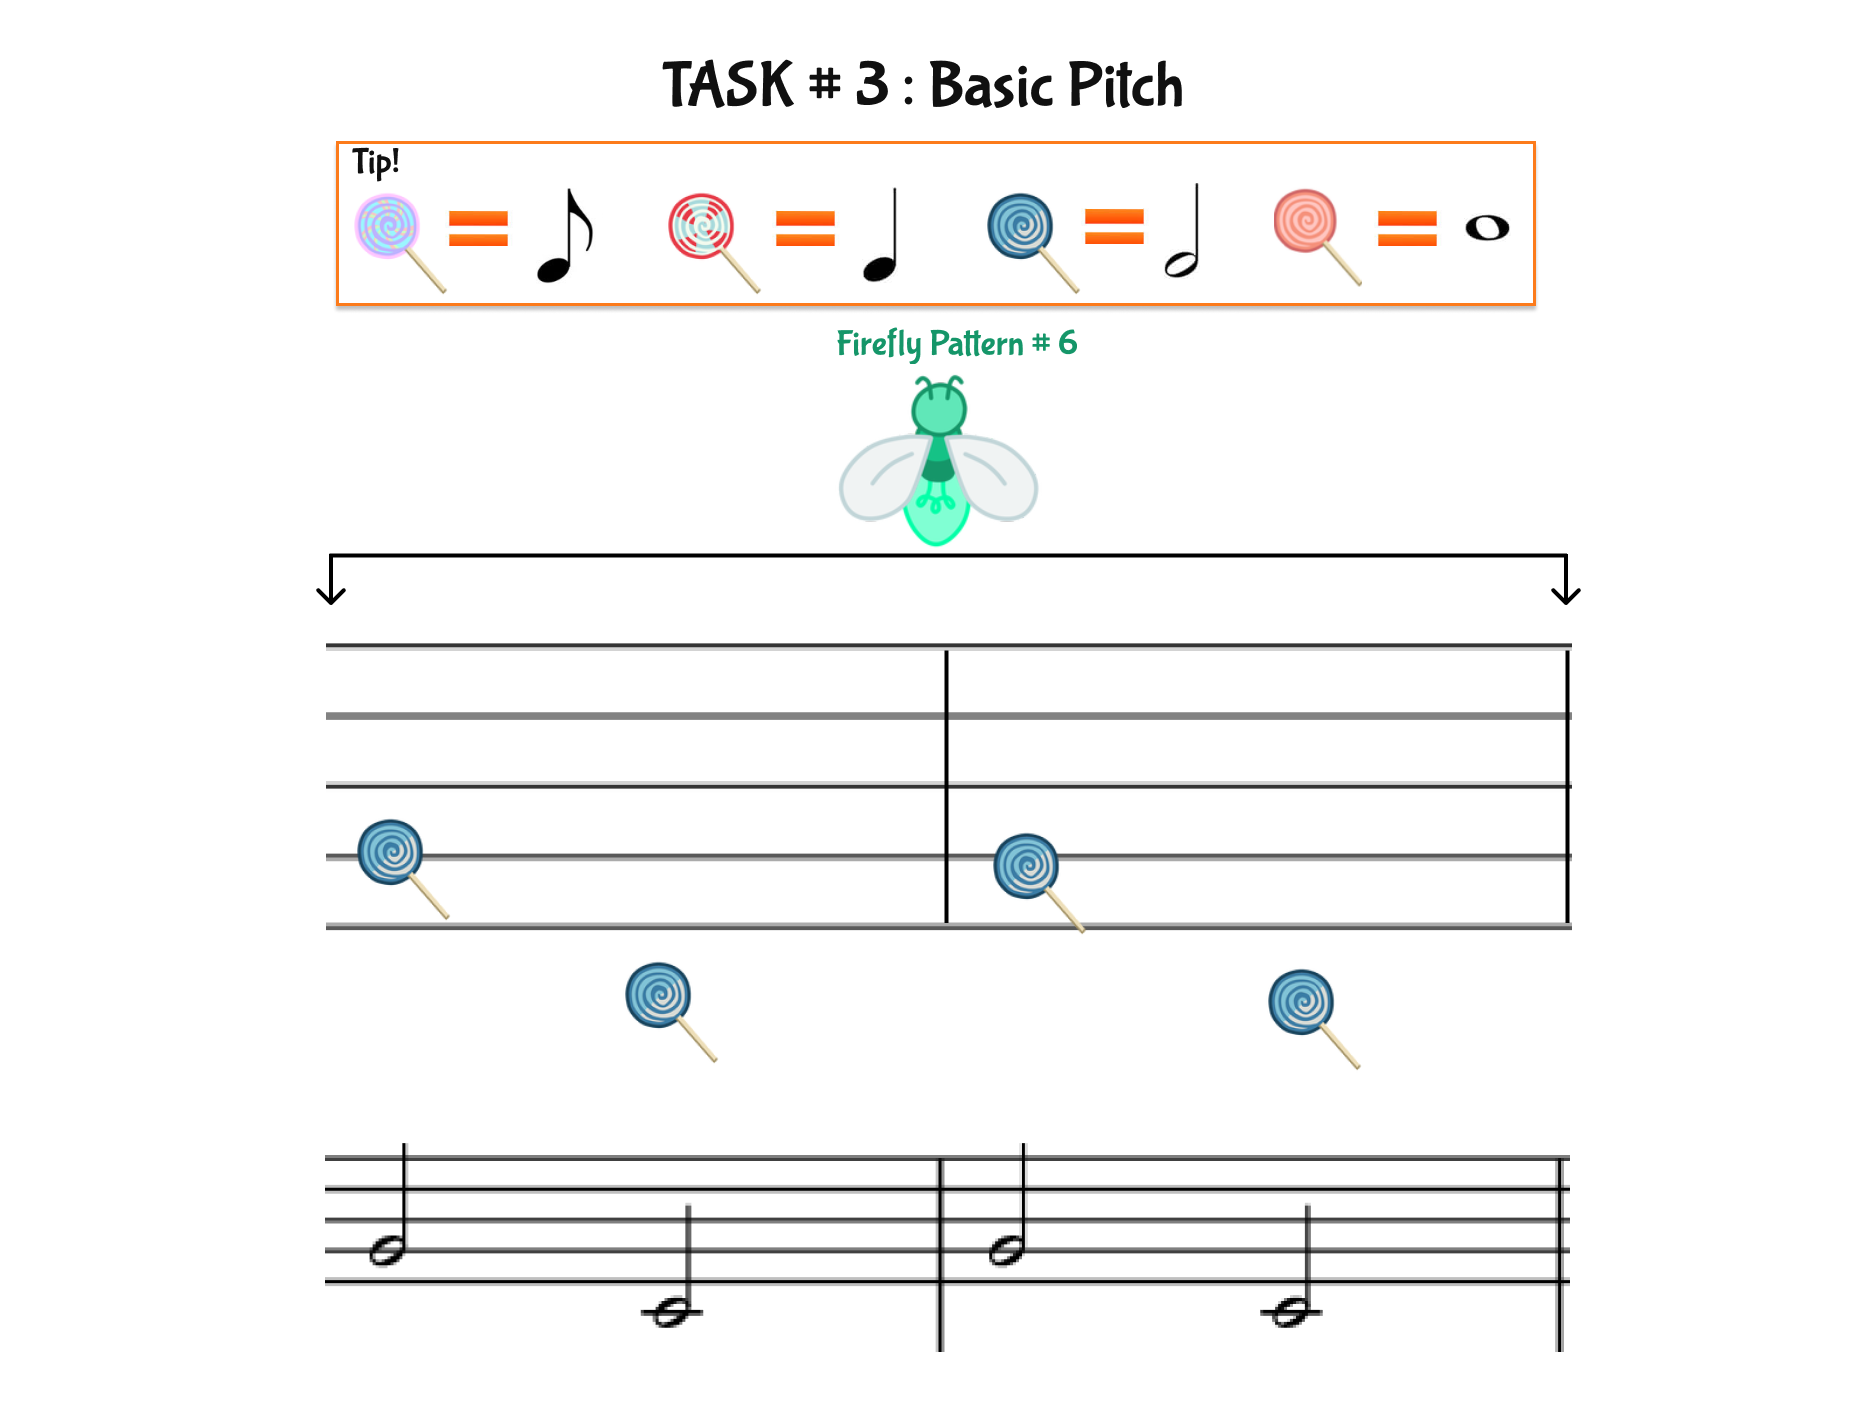
\includegraphics[width=12cm]{figures/NewFigures/BasicPitchTip6.png}
    \caption{Basic Pitch Tip 6}
    \label{fig:BasicPitchTip6}
\end{figure}

\begin{figure}[H]
    \centering
    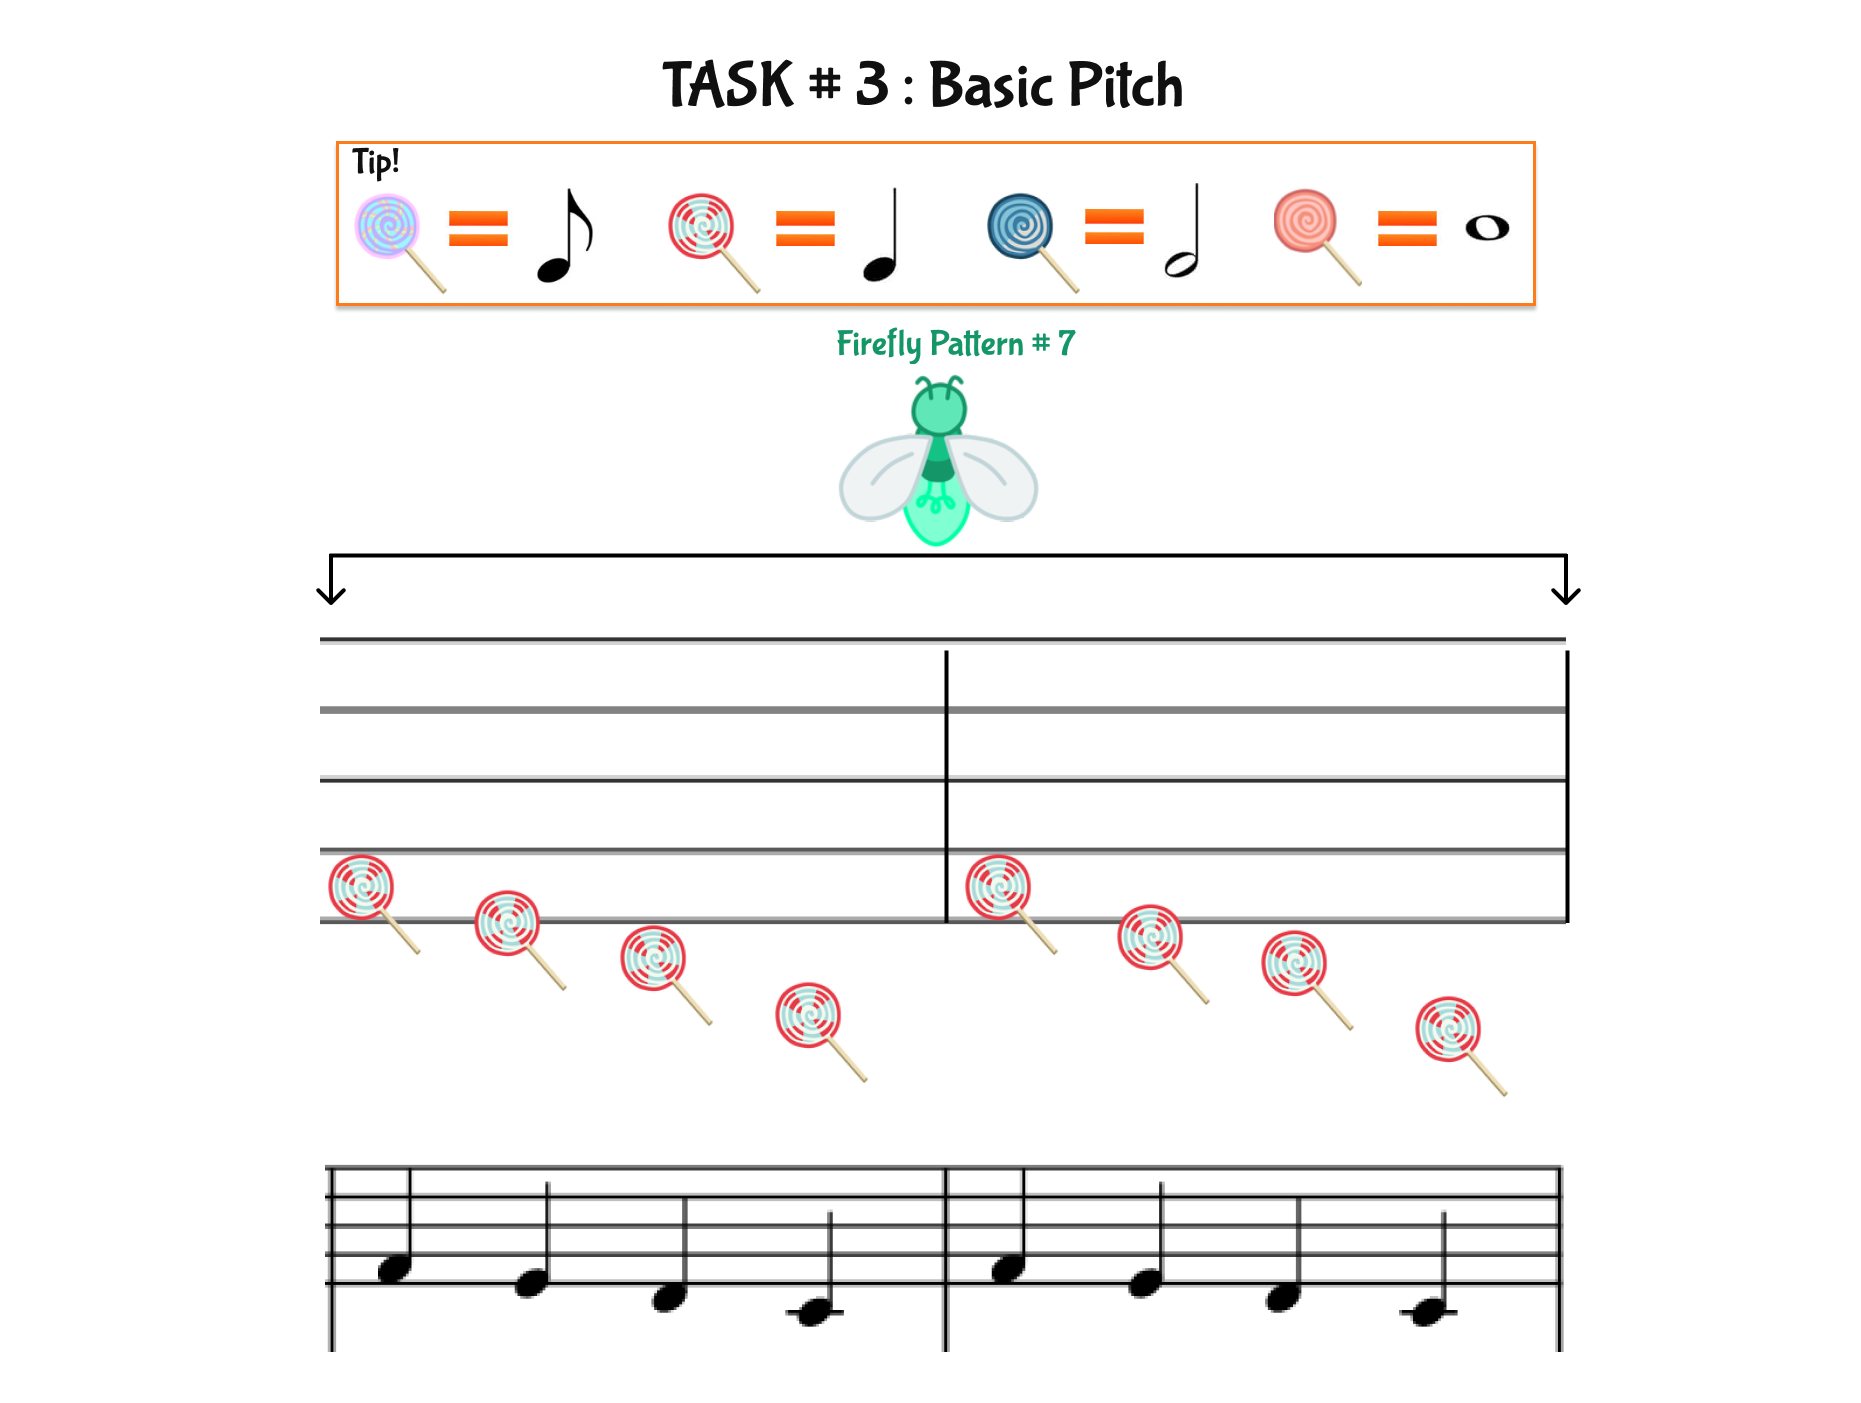
\includegraphics[width=12cm]{figures/NewFigures/BasicPitchTip7.png}
    \caption{Basic Pitch Tip 7}
    \label{fig:BasicPitchTip7}
\end{figure}

\begin{figure}[H]
    \centering
    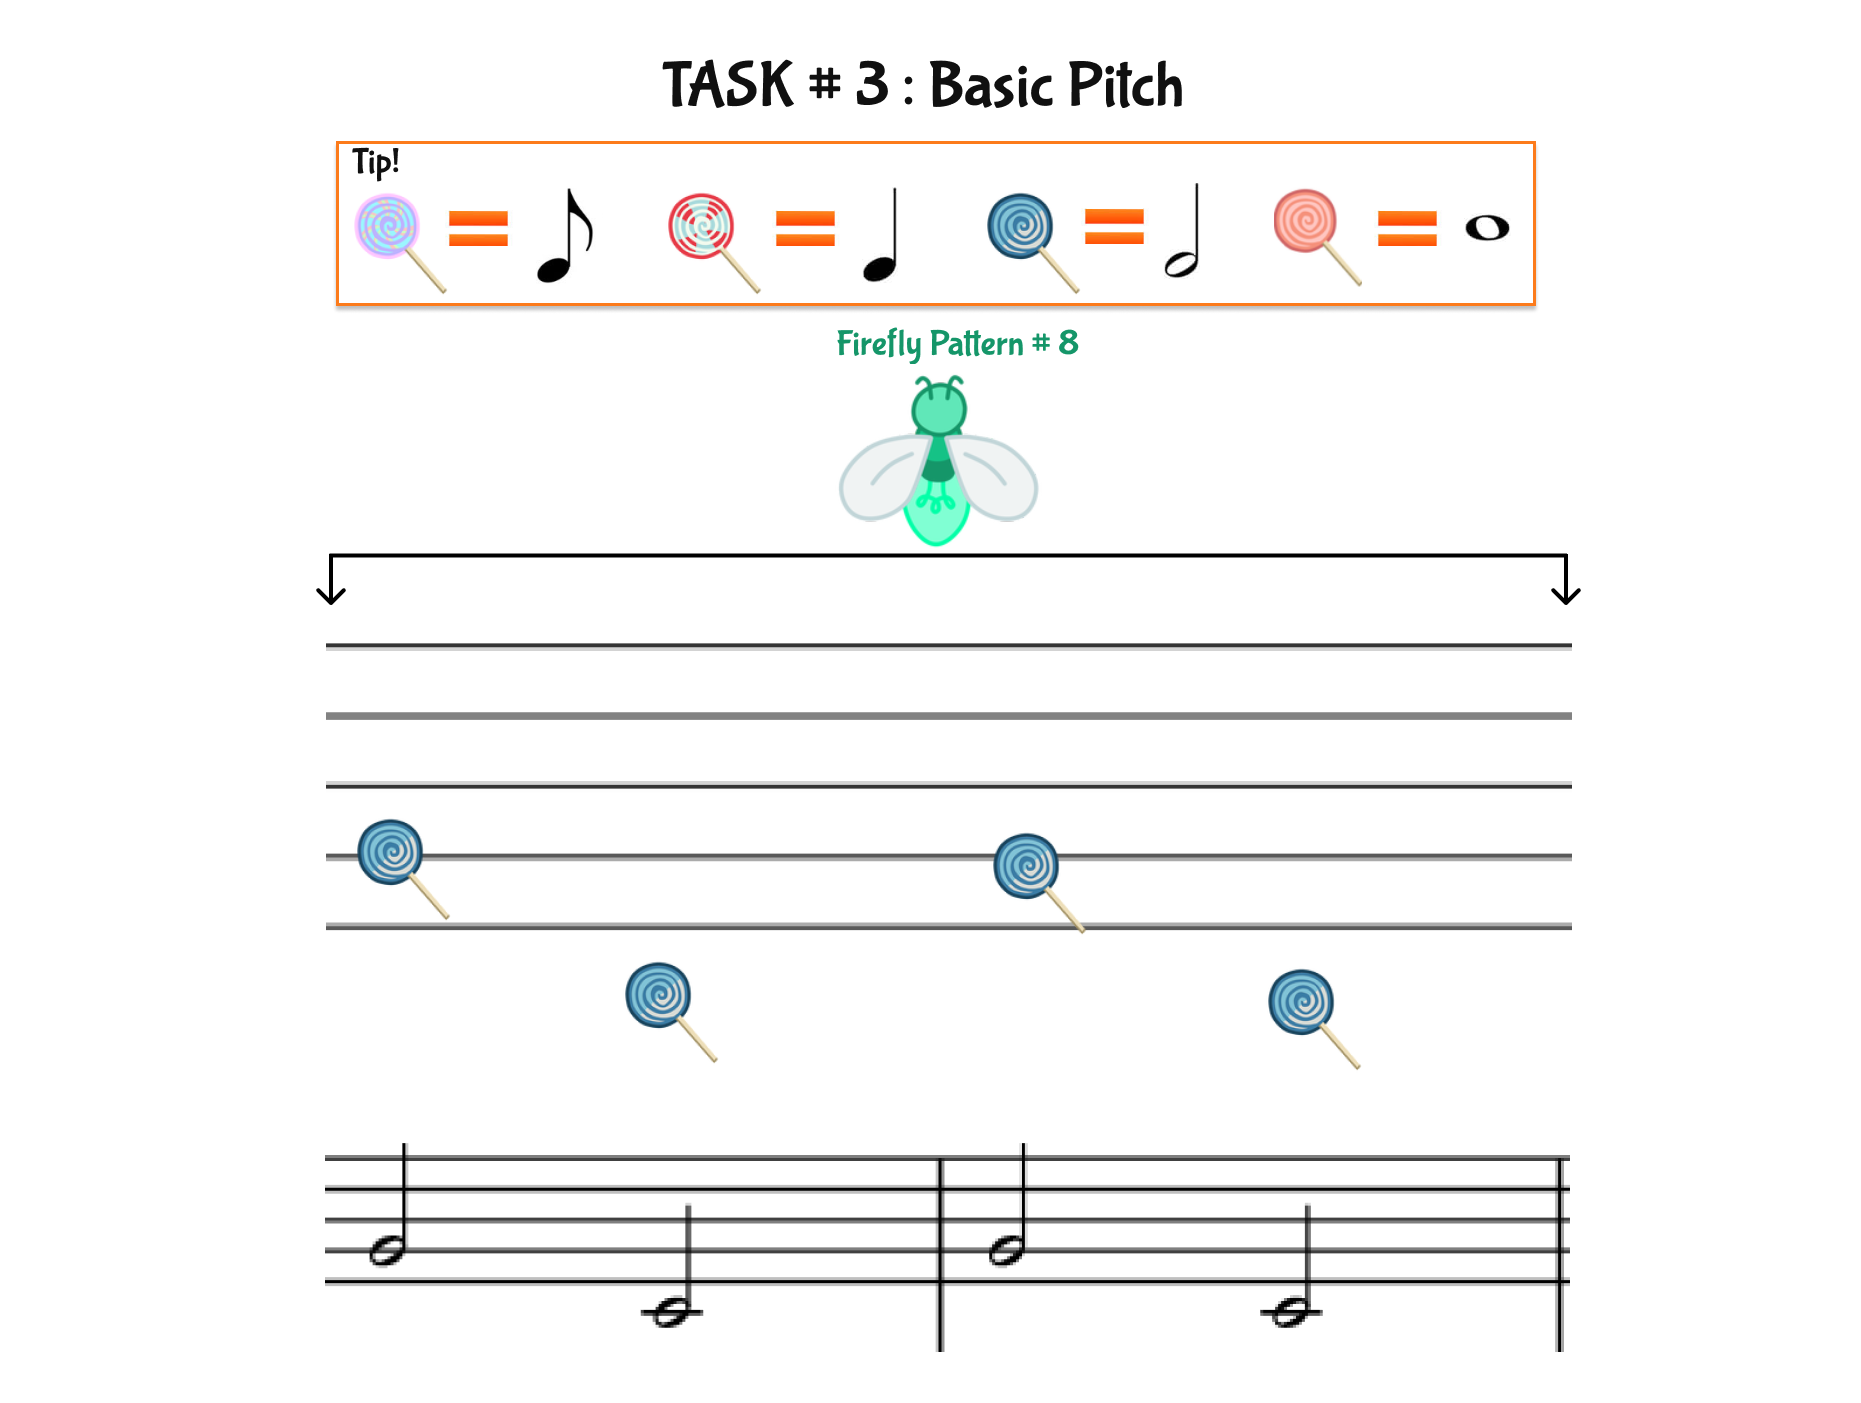
\includegraphics[width=12cm]{figures/NewFigures/BasicPitchTip8.png}
    \caption{Basic Pitch Tip 8}
    \label{fig:BasicPitchTip8}
\end{figure}

\begin{figure}[H]
    \centering
    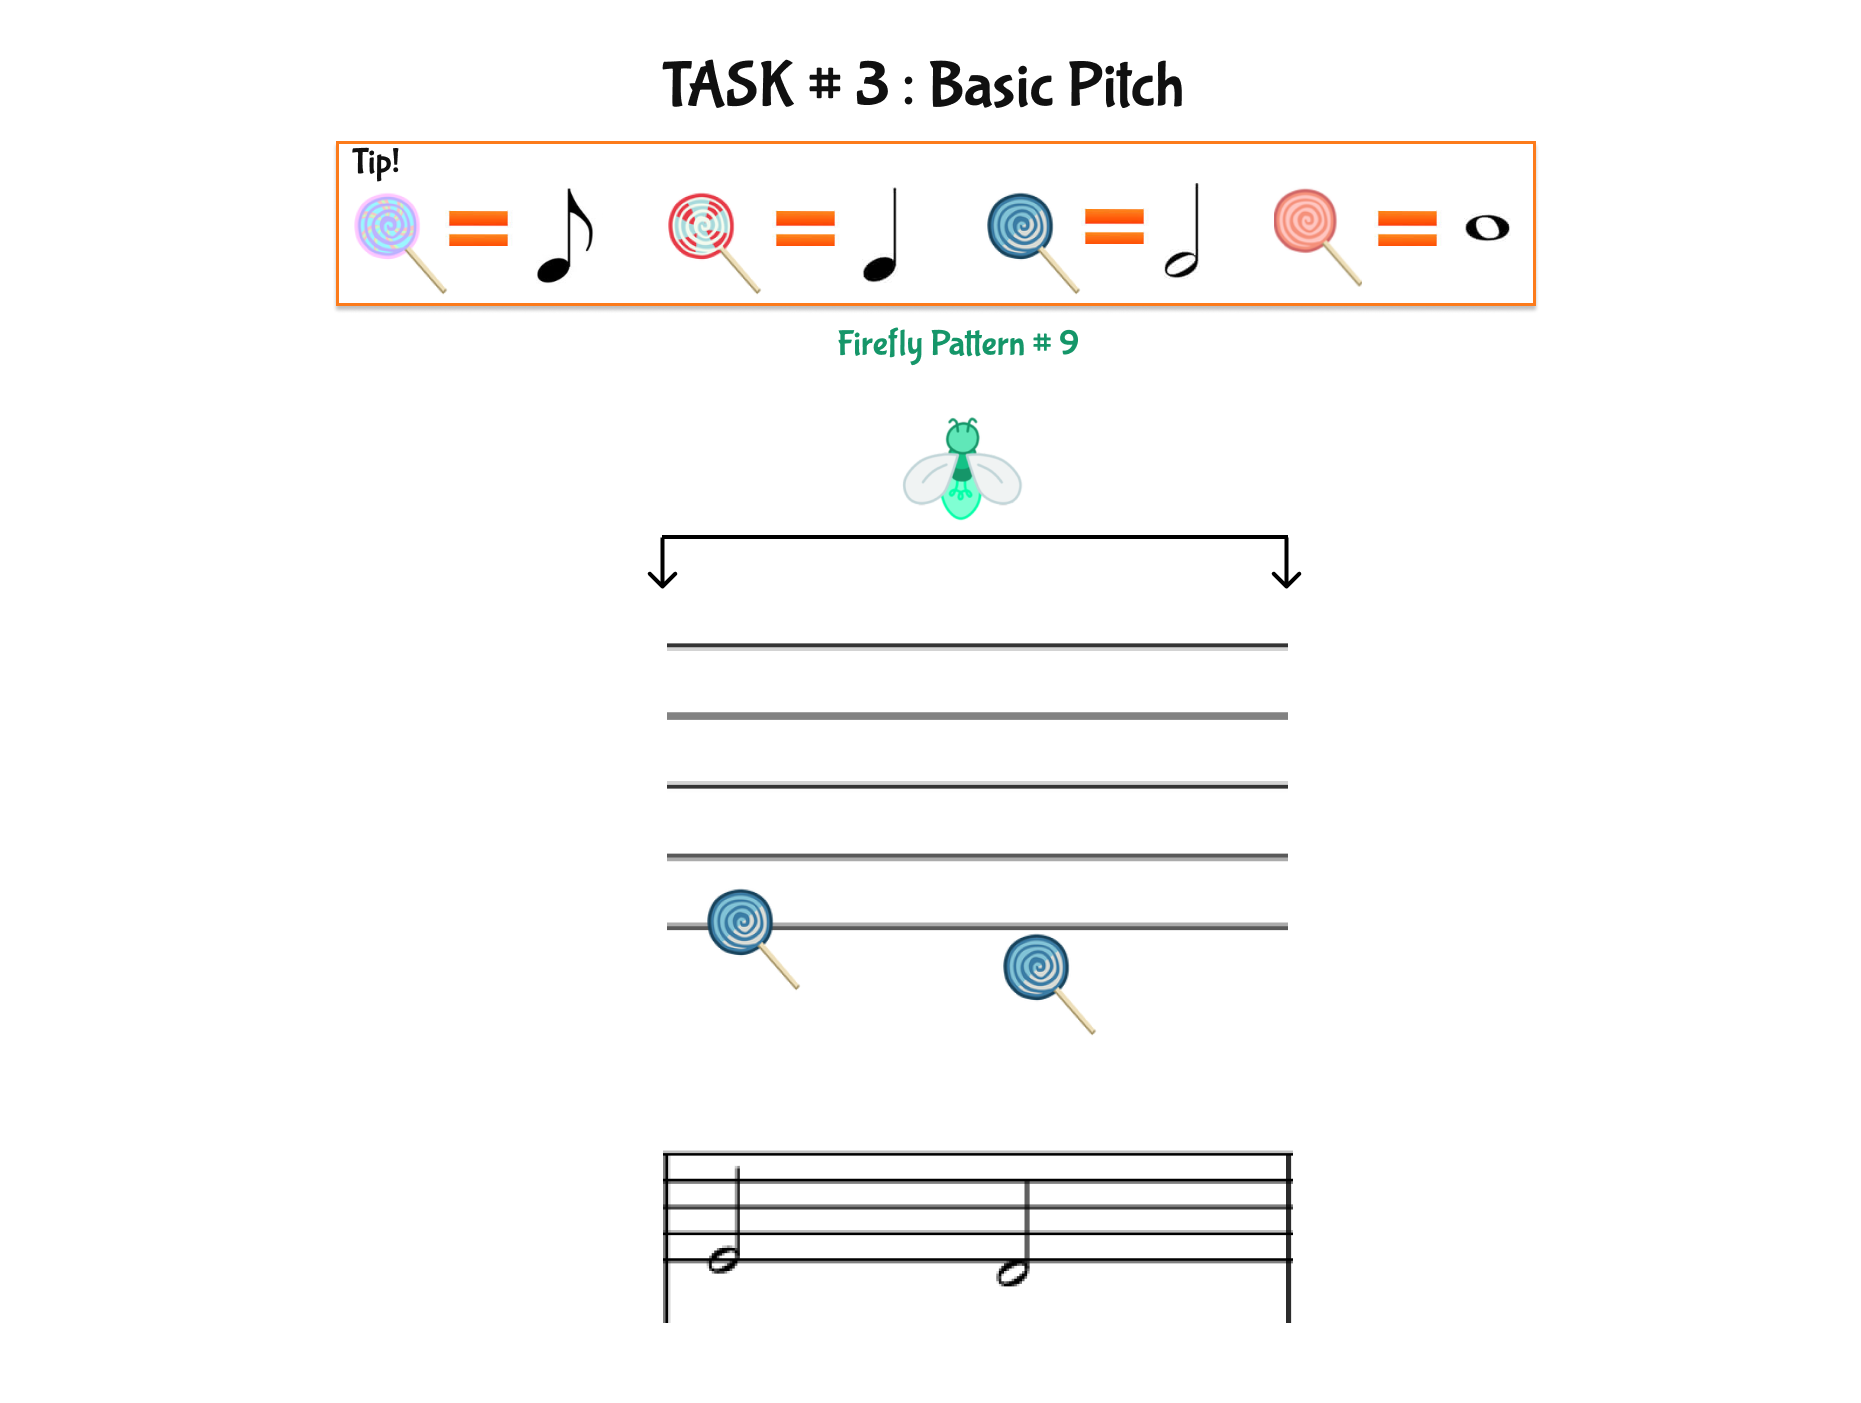
\includegraphics[width=12cm]{figures/NewFigures/BasicPitchTip9.png}
    \caption{Basic Pitch Tip 9}
    \label{fig:BasicPitchTip9}
\end{figure}

\begin{figure}[H]
    \centering
    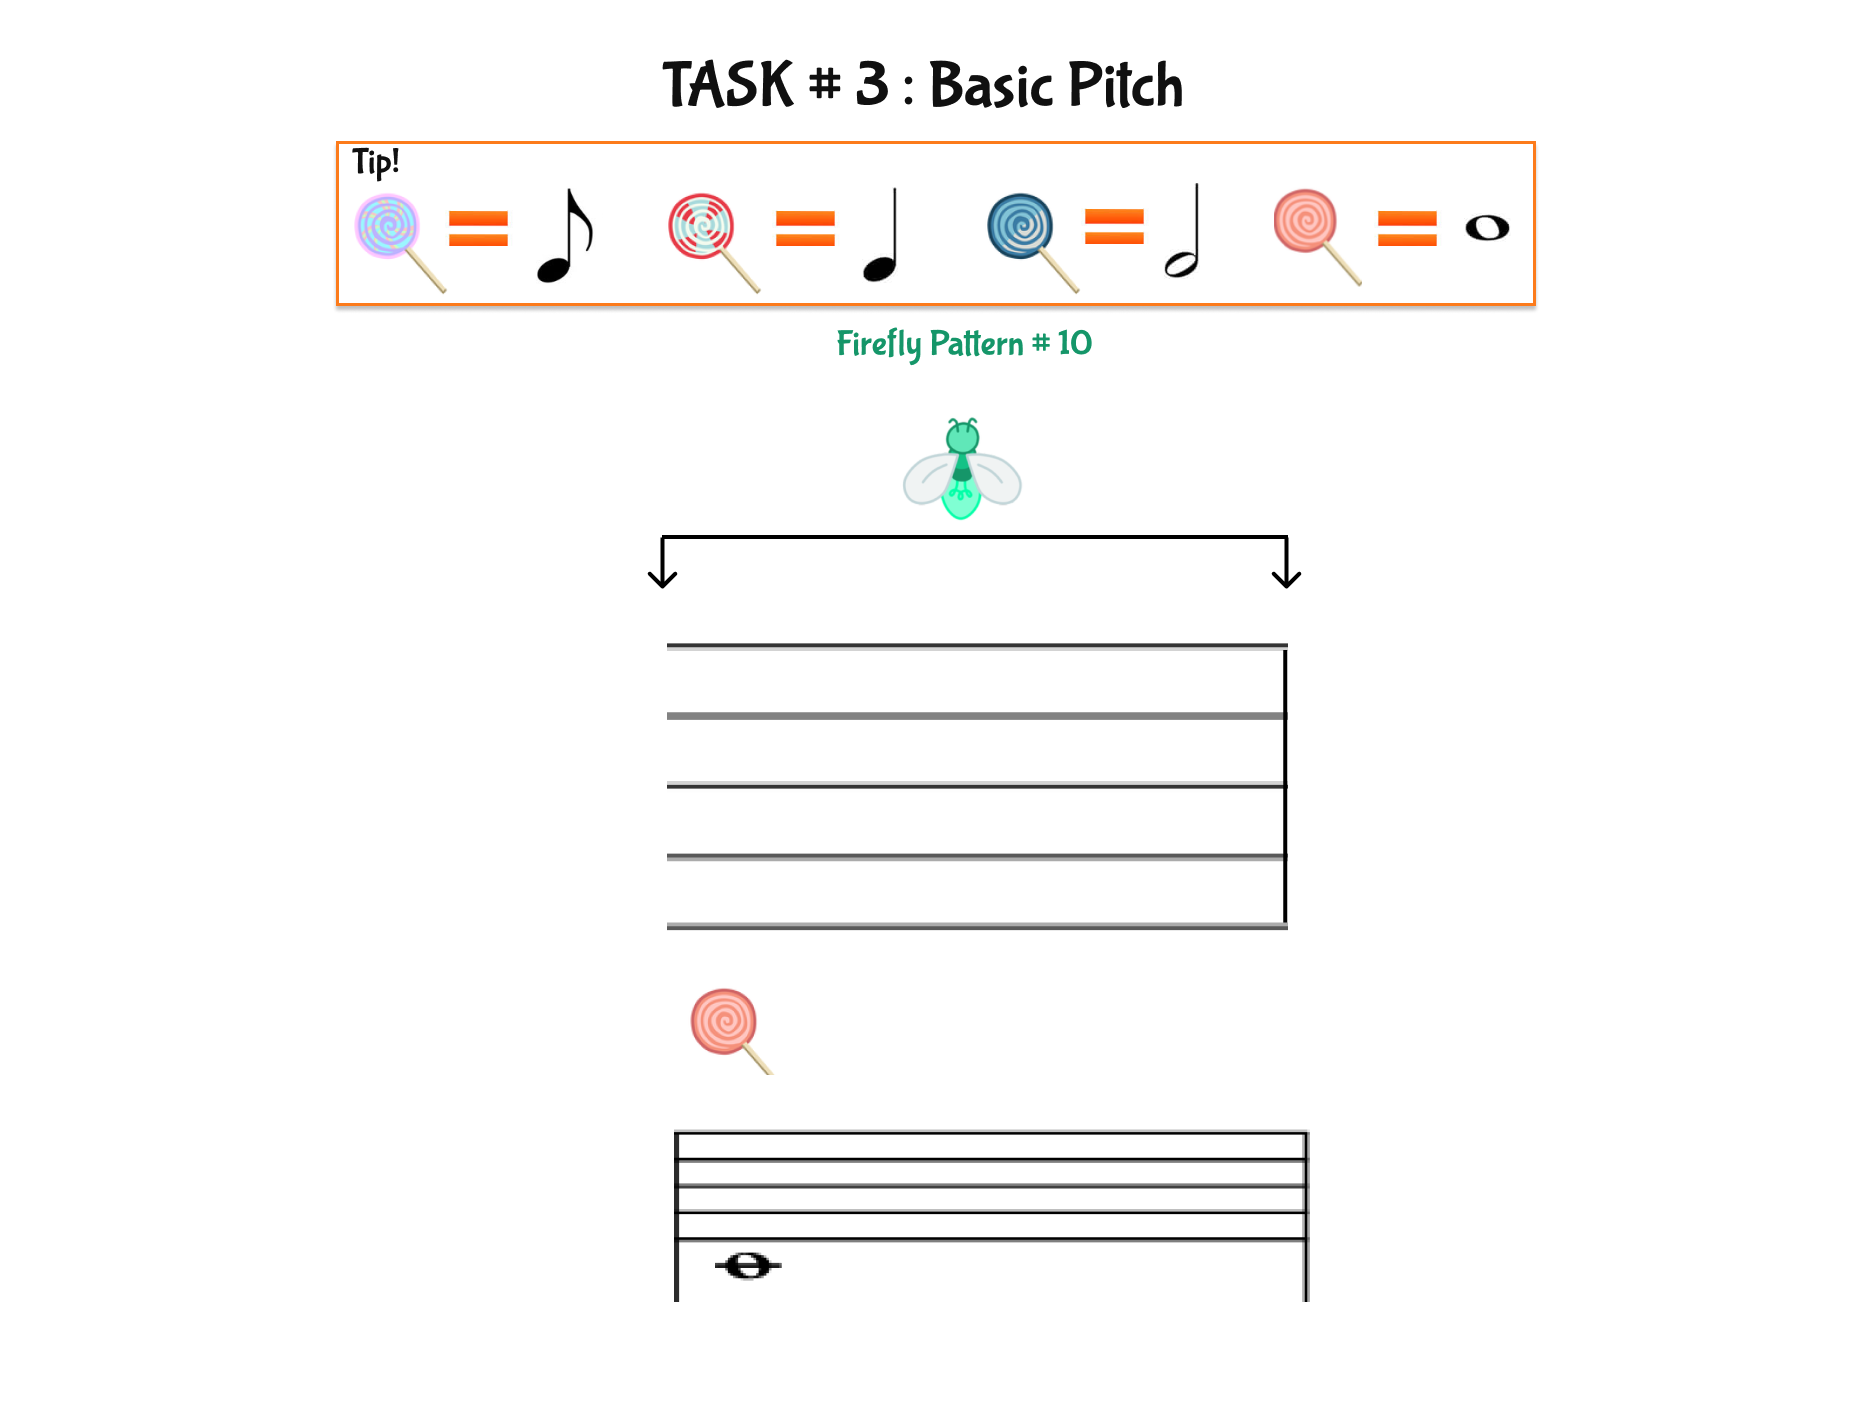
\includegraphics[width=12cm]{figures/NewFigures/BasicPitchTip10.png}
    \caption{Basic Pitch Tip 10}
    \label{fig:BasicPitchTip10}
\end{figure}

For the fourth task, the child is asked to recreate a part of the song \textit{"Twinkle Twinkle Little Star"} with a music sheet which could be seen in Figure \ref{fig:TTLSMusicSheet}, and an audio file that the child could listen to. Compared to task 2 and task 3, task 4 does not have the visual tips and. The child could only refer to the music sheet and the audio file to recreate the song. This task aims to help the child memorize the different music notes, patterns, and pitches. Like in the previous tasks, the guardians is expected to give minimal guidance and assurance to the child throughout the task. 

\begin{figure}[H!]
    \centering
    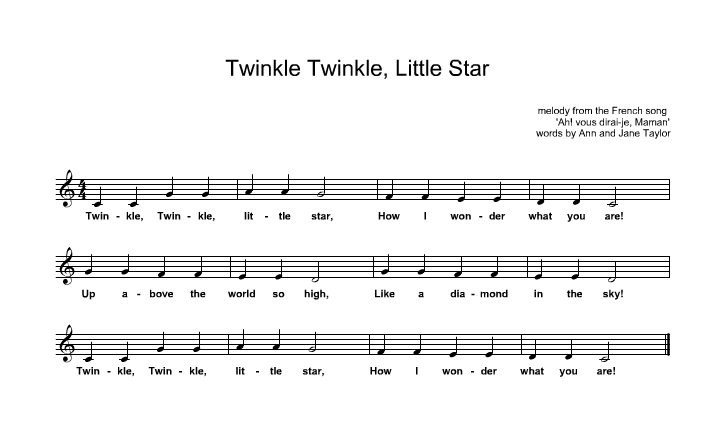
\includegraphics[width=15cm]{figures/NewFigures/TwinkleTwinkleLittleStarMusicSheet.png}
    \caption{Twinkle Twinkle Little Star Music Sheet}
    \label{fig:TTLSMusicSheet}
\end{figure}

The last task given to the child aims to assess how much of the music elements is memorized by them. In this task, the child is asked to compose a small part of the song \textit{"London Bridge is Falling Down"}. The music sheet for the song could be seen in Figure \ref{fig:LBIFDMusicSheet}. Unlike the previous tasks where the child is provided with music sheets and visual tips for task 2 and task 3, the last task provides only an audio file that the child could listen to. Like in the previous tasks, the guardians is also expected to give minimal guidance and assurance to the child throughout the task. 

During all of the sessions, the participants were asked to have their video on which all of their parents consented upon. They were also asked verbal consent for recording but participant 1 and participant 5 were not able to consent since they were not accompanied by a guardian during the sessions. We made use of the video and audio recordings to help us collect and observe various findings during the usability tests. 

\begin{figure}[H]
    \centering
    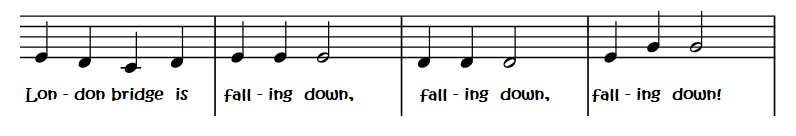
\includegraphics[width=15cm]{figures/NewFigures/LondonBridgeMusicSheet.png}
    \caption{London Bridge Is Falling Down Music Sheet}
    \label{fig:LBIFDMusicSheet}
\end{figure}


\section{Usability Test Results}
Quantitative data such as time completion per task, and number of assistance received by the participant per task were tracked during the sessions. Micro-interactions such as looking at their guardians for approval, asking something to their guardian, and the times the guardians gave assistance to the participant in any way were all recorded and added to get a total amount of assistance received by the participant. The total time taken by each participant per task could be seen in Figure \ref{fig:alltime}, and the total assistance received by each participant per task could be seen in Figure \ref{fig:allassistance}. P1 & P5 did not have a guardian during the sessions which is why they did not receive any kind of assistance while doing their tasks.

\begin{figure}[H]
    \centering
    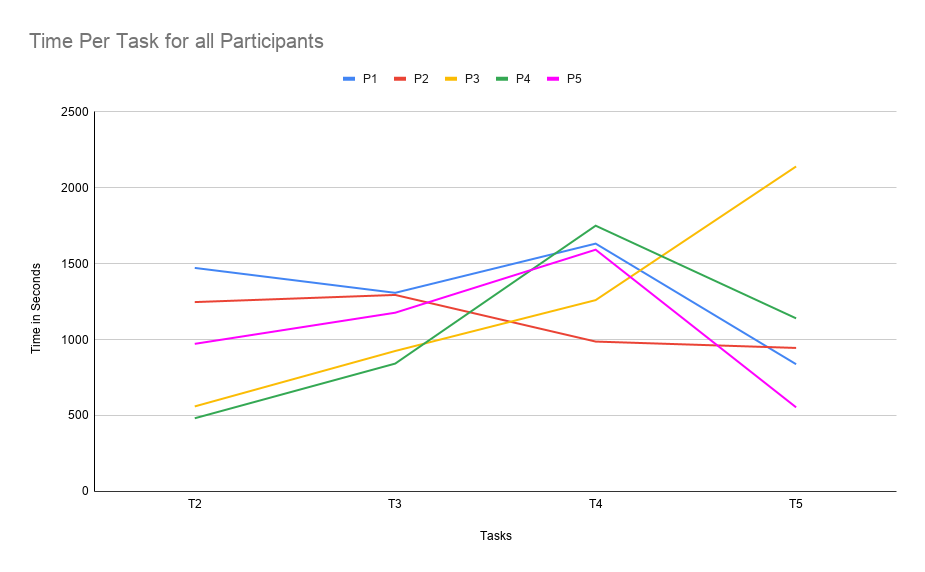
\includegraphics[width=15cm]{figures/Results/allParticipants.png}
    \caption{Time per Task for all Participants}
    \label{fig:alltime}
\end{figure}

\begin{figure}[H]
    \centering
    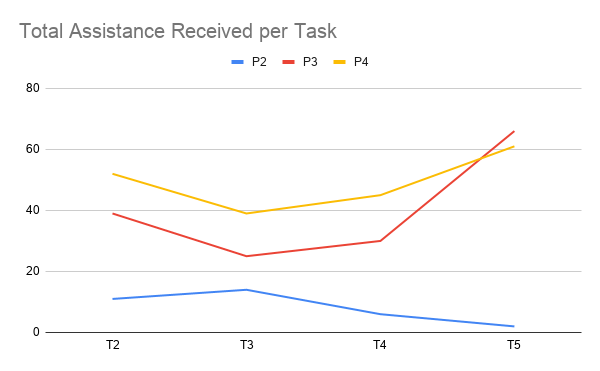
\includegraphics[width=15cm]{figures/Results/allAssistance.png}
    \caption{Total Assistance Received per Task for all Participants}
    \label{fig:allassistance}
\end{figure}

It can be seen in Figure \ref{fig:allassistance} that P2 received the least amount of assistance aside from P1 and P5 who received no assistance at all. We believe that children with higher age can do the tasks given to them with minimal assistance while children with lower age tend to rely more on their guardian. This can be said because P2 was able to finish the tasks with minimal assistance especially P1 and P5 with no assistance at all, while P3 and P4 needed a lot of assistance from their guardian. 

\begin{figure}[H]
    \centering
    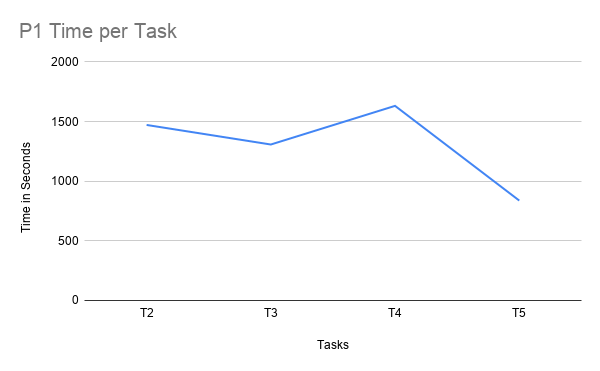
\includegraphics[width=15cm]{figures/Results/P1Time.png}
    \caption{Participant 1 Time per Task}
    \label{fig:P1Time}
\end{figure}

% In Figure \ref{fig:alltime}, it can be seen that only P1 took less time in doing T3 compared to T2. Based from our observations, P1 seems to have understood how to compose a song by following the tips given to him during T2 while other participants were getting familiar with the app during T3. 
In Figure \ref{fig:P1Time}, it can be seen that P1 took the longest time in T4 and the shortest time in T5. Based from our observations, P1 had difficulties in trying to compose a song using only a music sheet. This might be because when doing T3 and T2, P1 relied on the visual tips instead of the music sheet. We believe that T5 was too difficult for P1 because even though P1 knows that the output is wrong, P1 still decided to end the task.

\begin{figure}[H]
    \centering
    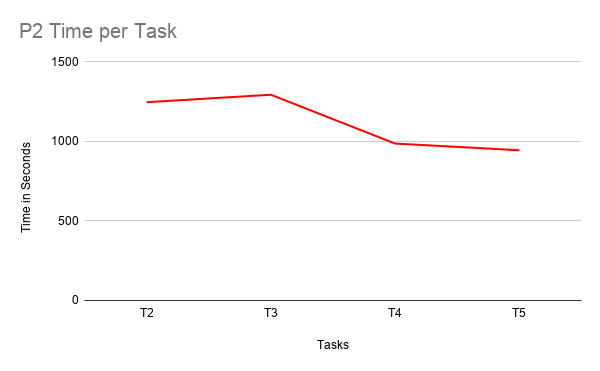
\includegraphics[width=15cm]{figures/Results/P2Time.png}
    \caption{Participant 2 Time per Task}
    \label{fig:P2Time}
\end{figure}

It can be seen in Figure \ref{fig:P2Time} that P2 took more time in doing T3 than T2. This might be because P2 was still learning the application during T3. P2 also took less time in doing T4 than T3. We observed that P2 was already familiar with the application and also familiar with how to read a music sheet which might be the reason why P2 finished T4 faster than T3. 

\begin{figure}[H]
    \centering
    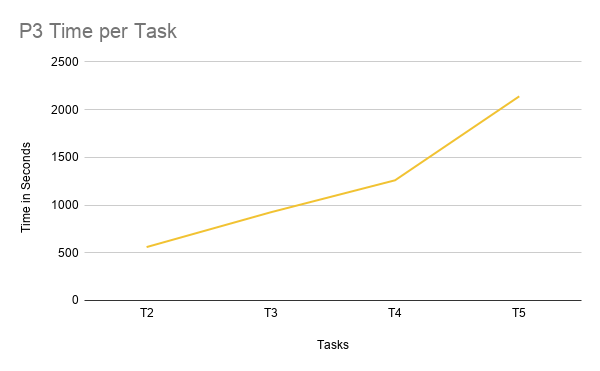
\includegraphics[width=15cm]{figures/Results/P3Time.png}
    \caption{Participant 3 Time per Task}
    \label{fig:P3Time}
\end{figure}

It can be seen in Figure \ref{fig:P3Time} that P3 had a faster time time in completing T1, this is because P3 received more assistance compared to P1 and P2. Particularly, P3 had only increasing time in the graph compared to the other participants. It can be seen that P3 was the only one with a time line that has a trend of going up, this is because P3 wanted to be correct so P3 used more time this might be why P3 was the only one to get task 5 correctly. 

\begin{figure}[H]
    \centering
    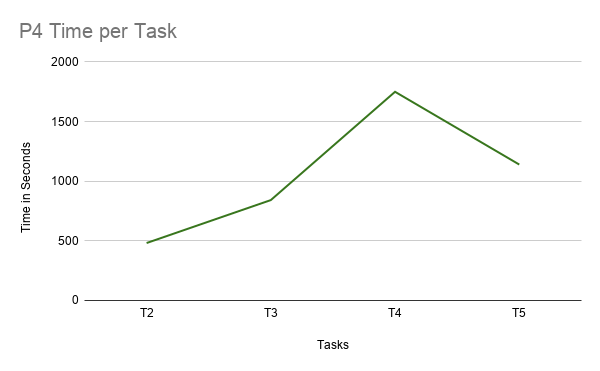
\includegraphics[width=15cm]{figures/Results/P4Time.png}
    \caption{Participant 4 Time per Task}
    \label{fig:P4Time}
\end{figure}

It can be seen in Figure \ref{fig:4Time} similar to P3, P4 had the fastest time in completing T1, this is because P4 received the most assistance compared to the other participants. Due to the assistance received P4 has a harder time in finishing T4 where we encouraged the parents to give no assistance. By T5, P4 was getting more confident in using the application this maybe the reason the time to complete was reduced.

\begin{figure}[H]
    \centering
    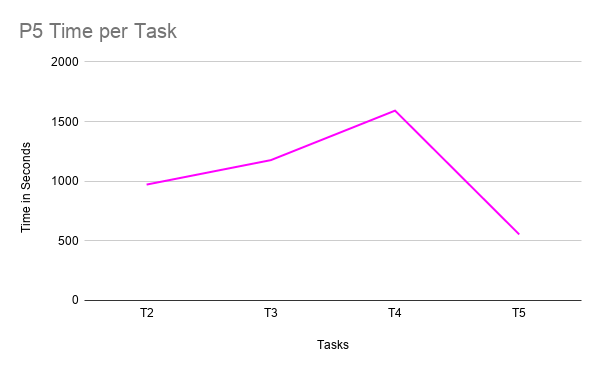
\includegraphics[width=15cm]{figures/Results/P5Time.png}
    \caption{Participant 5 Time per Task}
    \label{fig:P5Time}
\end{figure}

It can be seen in Figure \ref{fig:P5Time} that P5 also had a similar trend wherein they have increasing time as they are given harder tasks. The sudden decrease in time for T5 was because P5 decided to give up on finishing T5.

\section{AttrakDiff Results}
AttrakDiff is an instrument for measuring the attractiveness of interactive products. AttrakDiff makes use of pairs of opposite adjectives that users can choose from to indicate their perception of the product. These adjective-pairs make a collation of the evaluation dimensions possible. In the current version, AttrakDiff is able to measure the perceived pragmatic quality (PQ), perceived hedonic quality-identification (HQ-I), perceived hedonic quality-stimulation (HQ-S), and the attractiveness (ATT) of a product.

Pragmatic quality (PQ) describes the usability of a product and indicates  how successfully users are in achieving their goals using the product. Hedonic quality - stimulation (HQ-S) indicates to what extent the product can support the needs of the user in terms of interesting, and stimulating functions, and interaction- and presentation-styles. Hedonic quality - identity (HQ-I) indicates to what extend the product can allow the user to identify with it. And lastly, attractiveness (ATT) describes a global value of the product based on the quality perception.

%\subsection{AttrakDiff Protocol}
After the participant has finished the last task, they are asked to answer the AttrakDiff survey. The survey contains 28 different attributes which are categorized into PQ, HQ-S, HQ-I, and ATT. All the attributes are evaluated using a 7-scale method that represent opposites (good-bad). The middle value is 0, left-most value as -3 and right-most value as +3.  During the survey, the participants and their guardians might not be familiar with some word pairs. In this case, we try to explain the meaning of the word but reiterate to them that they have to choose the first word that comes into their mind.

%\subsection{AttrakDiff Results}
From the data collected, AttrakDiff was able to generate three diagrams. The first one is the Portfolio presentation which can be seen in Figure \ref{fig:PortfolioOfFireflyX}. The average word pair assessment values for pragmatic and hedonic qualities created a point on the map. The location of the point also showed in which area the point belonged to. The next diagram is the diagram of average values which can be seen in Figure \ref{fig:DiagramOfAverageValues}. In this diagram, the vertical axis represents  the  average  assessment  values  of  the  word  pairs inside each group and the horizontal axis shows the four word groups (PQ, HQ-I, HQ-S, ATT). The last diagram is a visual representation of the word pair values selected by the children which could be seen in Figure \ref{fig:DiagramOfWordPairs}. This helps us understand their evaluations for the application. Word pairs are in the vertical axis, whereas the assessment is in the horizontal axis. The values in the Figure represent the chosen option in the word pair, -3 referring to the leftmost and 3 to the rightmost part of the scale. 
\begin{figure}[H]
    \centering
    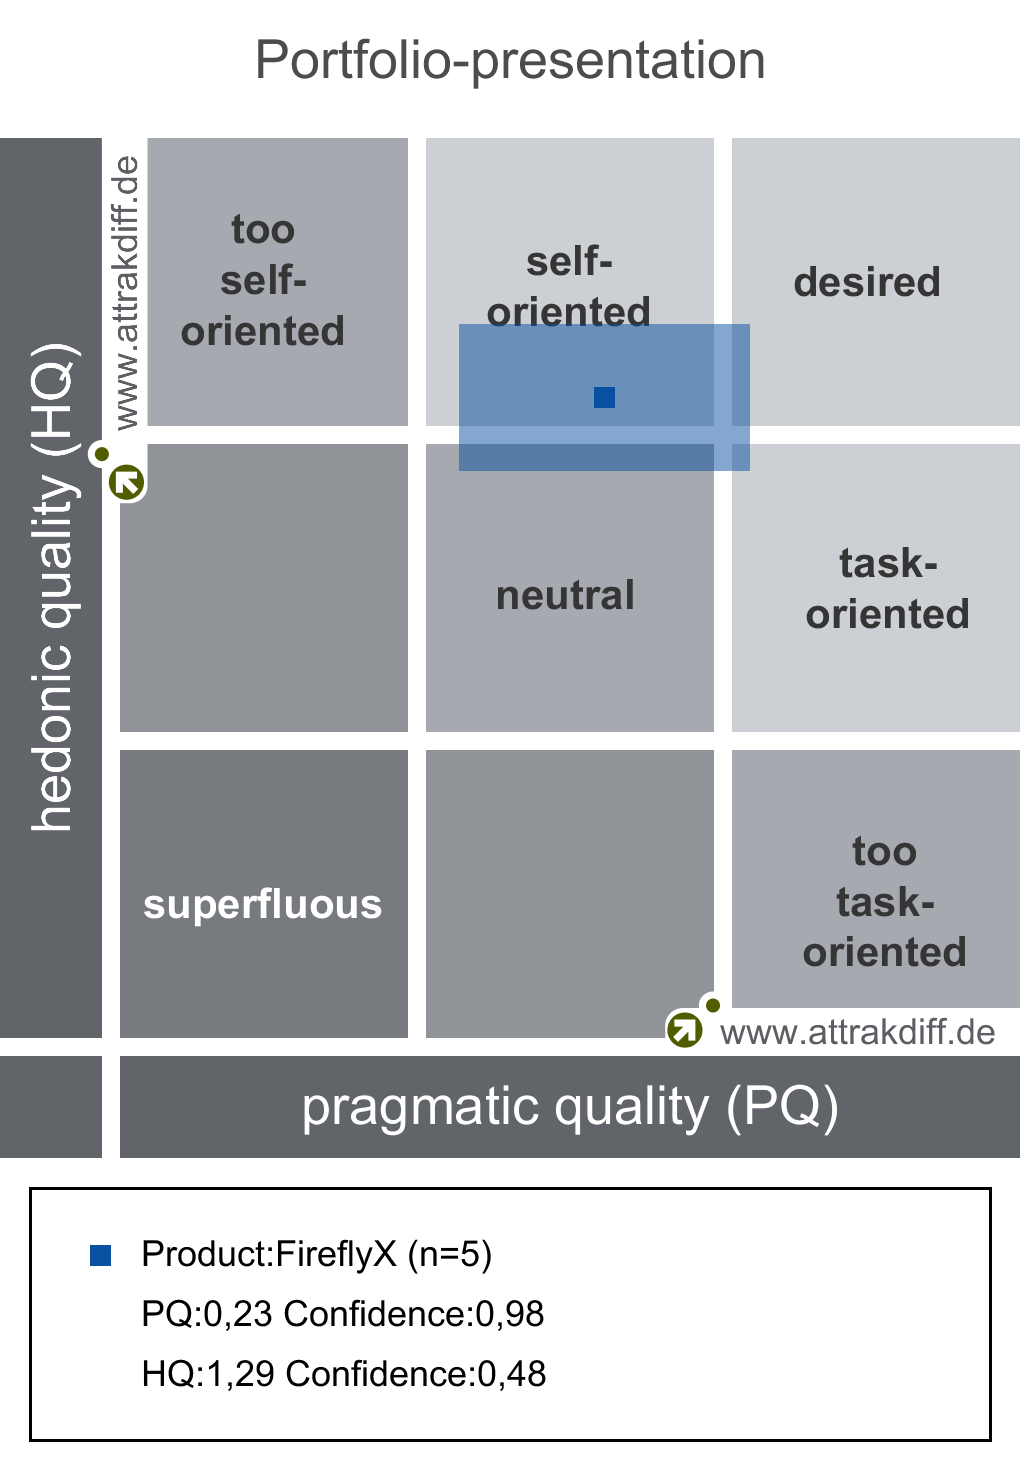
\includegraphics[width=11cm]{figures/NewFigures/Portfolio_of_results.png}
    \caption{Portfolio of FireflyX}
    \label{fig:PortfolioOfFireflyX}
\end{figure}

In Figure \ref{fig:PortfolioOfFireflyX} it can be seen that the graph produces a high value for the hedonic qualities and scored a little above average on the pragmatic qualities which indicates that the application has good usability and caters also to the interests of the children. The point on the graph lands on the "self-oriented" part which means features that enable the user to interact with other users are lacking.

\begin{figure}[H]
    \centering
    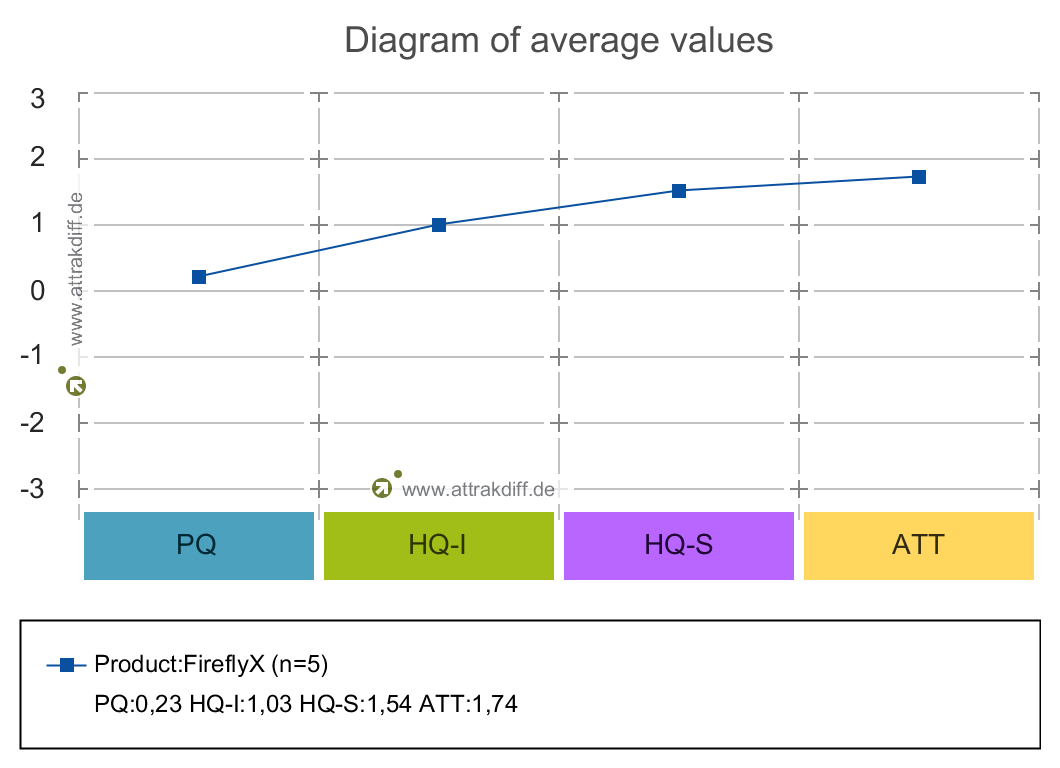
\includegraphics[width=14cm]{figures/NewFigures/Diagram_of_average_values.png}
    \caption{Diagram of Average Values}
    \label{fig:DiagramOfAverageValues}
\end{figure}

A bigger number on the y-axis depicts better UX with the didactic content, while a value that approximates to 0 expresses a neutral experience \cite{giardi2019evaluate}. It can be seen that all of the values are above 0. This indicates that the score for the usability of the application leans toward the neutral scale. While the hedonic qualities and the overall attractiveness of the application scored 1 and higher which means that the overall design caters to children.

\begin{figure}[H]
    \centering
    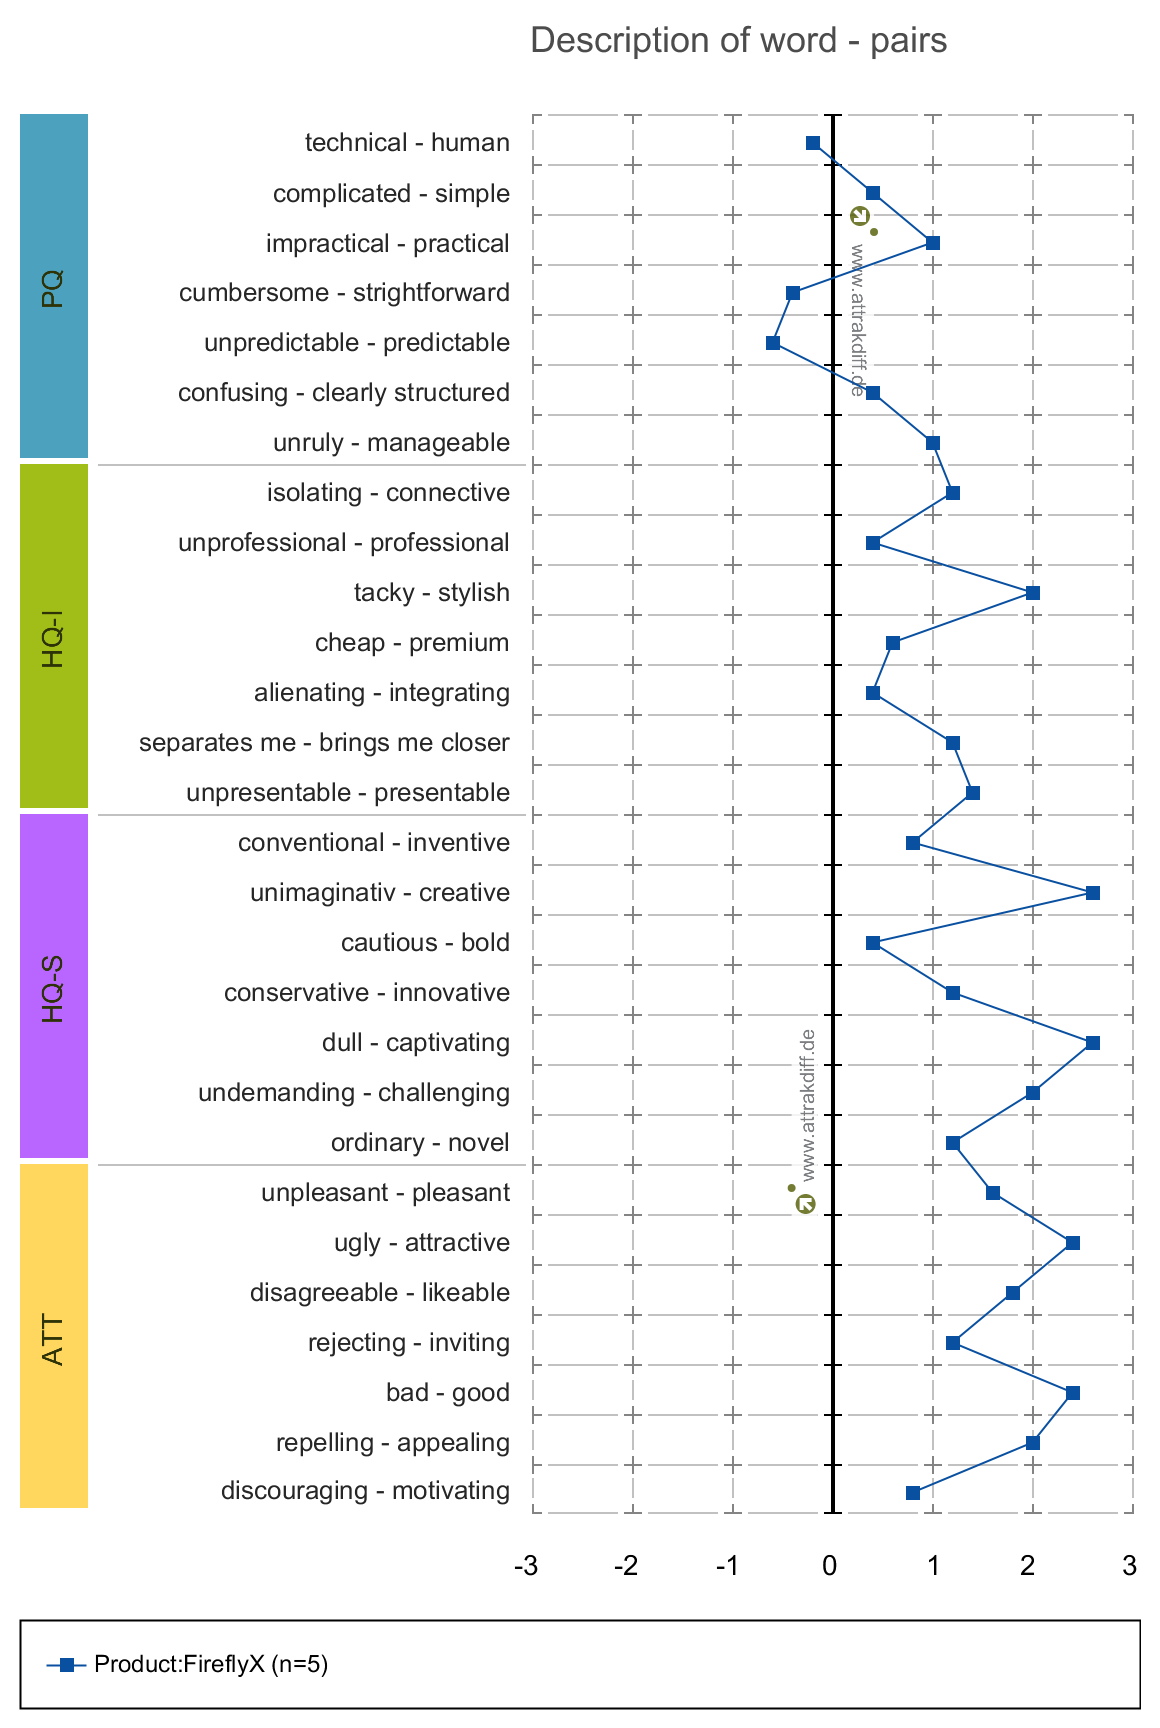
\includegraphics[width=12cm]{figures/NewFigures/Description_of_word-pairs.png}
    \caption{Diagram of Word Pairs}
    \label{fig:DiagramOfWordPairs}
\end{figure}

Figure \ref{fig:DiagramOfWordPairs} gives a more descriptive and in-depth answers of the participants. Here, specific values can be seen and what the score is for that word pair. As seen in the figure, words such as stylish, creative, captivating, and attractive were chosen by the participants instead of their counterparts. This is because the participants mentioned during the testing that they liked the design of the application. Words such as technical, cumbersome, and unpredictable were chosen because we observed that most of the participants were confused and had no idea how to use the application at the start.

\section{Expert Evaluation}
\subsection{Music Expert Demographics}
A total of five (5) music experts were recruited to participate in our research. As a pre-requisite, they needed to have at least six years of experience with music theory by the time they participated. The demographics of these experts can be seen in Table \ref{MusicExpertDemographic}.

\begin{table}[H]
\centering
\begin{tabular}{|l|l|} 
\hline
Characteristic  & Total(n=3)    \\ 
\hline
Age (mean \pm   SD [range]) & 21.7 \pm    1.5 [20-23]              \\ 
\hline
\begin{tabular}[c]{@{}l@{}}Sex (n [\%])\\~~~ Male\\~~~ Female\end{tabular}                                                 & \begin{tabular}[c]{@{}l@{}} 2 [33.3]\\1 [66.7]\end{tabular}                 \\ 
\hline
Years of Experience (mean \pm   SD [range])                                                                                    & 13 \pm    1 [12-14]                                                          \\ 
             
\hline
\begin{tabular}[c]{@{}l@{}}Specialty (n [\%])\\~~~ Classical Guitar\\~~~ Piano\\~~~ Instrumentalist\end{tabular}                  & \begin{tabular}[c]{@{}l@{}} 1 [33.3]\\1 [33.3]\\1 [33.3]\end{tabular}  \\ 
\hline
\end{tabular}
\caption{Music Experts Demographic}
\label{MusicExpertDemographic}
\end{table}


%\subsection{Expert Evaluation Protocol}
Similar to the testing with the participants, meeting with the music experts in person is also not viable due to the covid-19 pandemic. This meant that we would have to send them the necessary files online. Because of this, we would also not be able to observe them while they are assessing the outputs of the participants. After the participants finished their tasks, we compiled a Google Drive that contained a profile of each of the participants, their output per task, the expected output per task, and the observations we had per task.

Like the participants, the music experts were also given an orientation about the research, the tasks given to the participants, and what we would ask them to do. After the orientation, we gave them a Google Forms link that contained questions about their demographic, an assessment form for each task, and a input field where they could put their comments and remarks about the output of the participant.

The assessment form is a subset from a music performance adjudication set created by \citeA{wrigley2013ecological}. It consists of the criteria pitch, rhythm, tempo, and memory. Each criterion had to be rated on a 7-point Likert scale from needs attention to excellent. Pitch relates to how accurate the pitch of the output is. Rhythm also relates to how accurate the rhythm is. This is the same for tempo, while the memory relates to how the participants remember the music.

%\subsection{Expert Evaluation Results}
After the music experts filled out the form, we created five graphs out of the data from the form. The graphs that we were able to make were the sum of an average scores per task of every participants, average pitch scores per task per participant, average rhythm scores per task per participant, average memory scores per task per participant, and average tempo scores per task per participant. We used these results to find trends that would be significant in order for us to find relationships with our qualitative and quantitative data.

\begin{figure}[H]
    \centering
    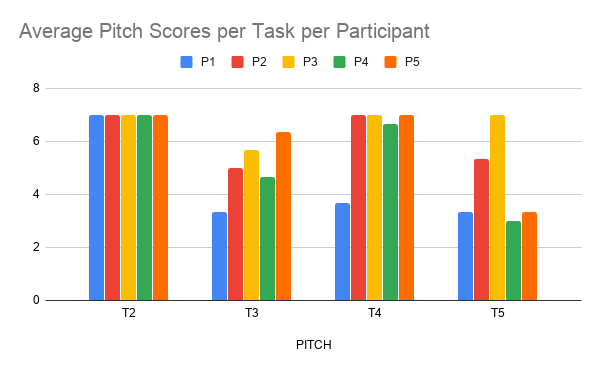
\includegraphics[width=11cm]{figures/Results/AveragePitch.png}
    \caption{Average Pitch Scores of Each Participant per Task}
    \label{fig:AveragePitch}
\end{figure}

As seen in Figure \ref{fig:AveragePitch}, T2 have equal scores as there is no pitch yet introduced in the task as it focused on the rhythm only. We can see that from T3 to T4 we see a big improvement in the scores of their pitch. This may be because they were still learning which notes correspond to the candies. We see a decrease in score from T4 to T5 because we think that they were relying on the music sheet guides in the previous tasks as compared to T5 where there was only a song for the guide. 

\begin{figure}[H]
    \centering
    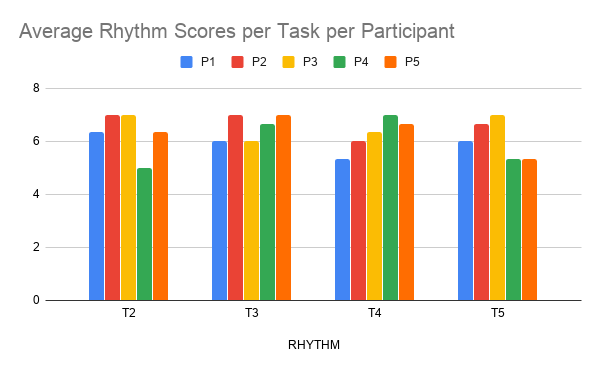
\includegraphics[width=11cm]{figures/Results/AverageRhythm.png}
    \caption{Average Rhythm Scores of Each Participant per Task}
    \label{fig:AverageRhythm}
\end{figure}

As seen in Figure \ref{fig:AverageRhythm}, the results are similar per task. Though in T5, we can see that P4 and P5 have lower score because they just accepted their mistake and decided to finish the task.

\begin{figure}[H]
    \centering
    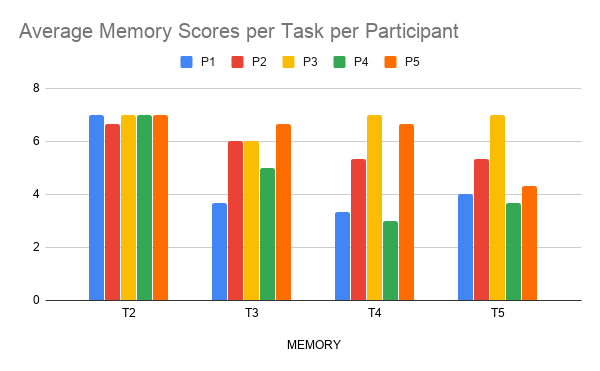
\includegraphics[width=11cm]{figures/Results/AverageMemory.png}
    \caption{Average Memory Scores of Each Participant per Task}
    \label{fig:AverageMemory}
\end{figure}

In Figure \ref{fig:AverageMemory}, it can be seen that P1 had trouble in T3, T4, and T5 in terms of memory. This is also true for P4 in T4, and T5. This might be because the expected outputs for T4, and T5 is quite different from what they are taught. 
% N O T A B L Y

\begin{figure}[H]
    \centering
    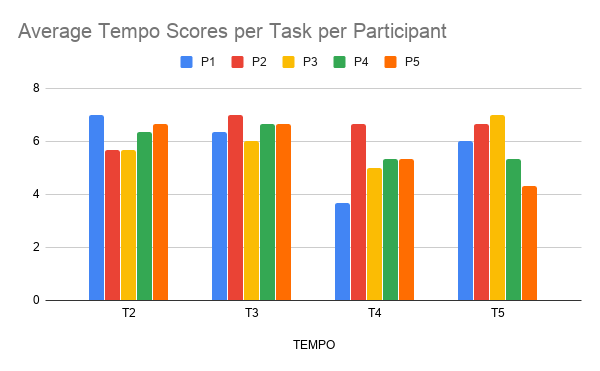
\includegraphics[width=11cm]{figures/Results/AverageTempo.png}
    \caption{Average Tempo Scores of Each Participant per Task}
    \label{fig:AverageTempo}
\end{figure}

As seen in Figure \ref{fig:AverageTempo}, it can be seen that the results for T2 and T3 are similar because the guides for both tasks included visual diagrams that showed the colors needed for the output. T4 noticeably had lower scores because the guide only included the music sheets and the music playback. Notably, one of the comments of our experts mentioned that children tend to choose slower tempos because it was the tempo that was taught to them in their earlier years of childhood.

\begin{figure}[H]
    \centering
    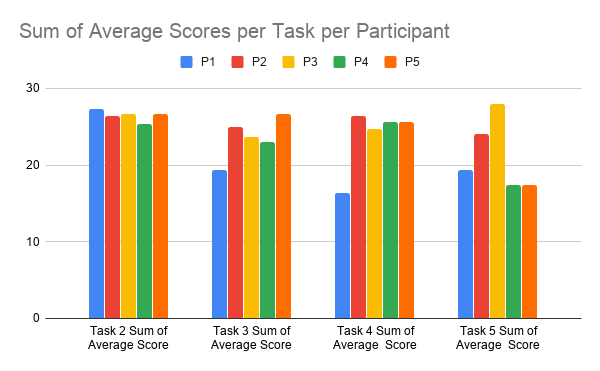
\includegraphics[width=11cm]{figures/Results/SumOfTotalAverage.png}
    \caption{Sum of Averages of Each Participant per Task}
    \label{fig:SumOfTotalAverage}
\end{figure}

It can be seen in Figure \ref{fig:SumOfTotalAverage} that the participants scored high in T2. Since T2 aims to teach rhythm to the participants, only rhythm scores and tempo scores are emphasized. It is also notable that P1, P4, and P5 scored relatively low because they settled for a wrong composition, while P2 and P3 did their best to ensure that what they composed were correct. Most of the participants had decreased score on T5 because the task had no other guides aside from the music playback.
